% !TeX program = xelatex
% XeLaTeX is recommended; pdfLaTeX and LuaLaTeX are supported too.
\documentclass[12pt,a4paper,oneside]{report}
\usepackage[left=25mm,right=23mm,top=23mm,bottom=24mm,headheight=15pt]{geometry}
\usepackage{iftex}
\ifPDFTeX
  % Type 1 editions of the same font families work with pdfLaTeX.
  \usepackage[T1]{fontenc}
  \usepackage[utf8]{inputenc}
  \usepackage{tgpagella,tgheros}
  \usepackage[scale=0.88]{tgcursor}
\else
  % OpenType font configuration for XeLaTeX, LuaLaTeX and Tectonic.
  \usepackage{fontspec}
  \setmainfont{texgyrepagella-regular.otf}[BoldFont=texgyrepagella-bold.otf,ItalicFont=texgyrepagella-italic.otf,BoldItalicFont=texgyrepagella-bolditalic.otf]
  \setsansfont{texgyreheros-regular.otf}[BoldFont=texgyreheros-bold.otf,ItalicFont=texgyreheros-italic.otf]
  \setmonofont{texgyrecursor-regular.otf}[BoldFont=texgyrecursor-bold.otf,ItalicFont=texgyrecursor-italic.otf,BoldItalicFont=texgyrecursor-bolditalic.otf,Scale=0.88]
\fi
\usepackage{amsmath,amssymb,booktabs,longtable,tabularx,array,graphicx,xcolor}
\usepackage{fancyhdr,titlesec,enumitem,listings,needspace,etoolbox,xurl,ragged2e}
\usepackage[protrusion=true,expansion=false]{microtype}
\usepackage[unicode,colorlinks=true,linkcolor=navy,urlcolor=teal,citecolor=navy]{hyperref}
\definecolor{navy}{HTML}{17324D}
\definecolor{teal}{HTML}{277D77}
\definecolor{muted}{HTML}{526371}
\definecolor{wash}{HTML}{F1F4F7}
\definecolor{rulegray}{HTML}{D2DCE3}
\hypersetup{pdftitle={Understanding SafeSliceSQL: A Beginner's Walkthrough},pdfauthor={Prepared from the SafeSliceSQL repository},pdfsubject={A first-principles walkthrough with a worked shop example, gradual explanations and a file-by-file reading guide},bookmarksnumbered=true}
\AtBeginDocument{\RaggedRight}
\setlength{\parindent}{0pt}
\setlength{\parskip}{8pt}
\linespread{1.08}
\setlength{\emergencystretch}{3em}
\setlength{\tabcolsep}{3pt}
\renewcommand{\arraystretch}{1.15}
\AtBeginEnvironment{longtable}{\small}
\setlist[itemize]{leftmargin=1.5em,itemsep=3pt,topsep=4pt}
\setlist[enumerate]{leftmargin=1.8em,itemsep=4pt,topsep=4pt}
\titleformat{\chapter}[display]{\sffamily\bfseries\color{navy}}{\large\chaptertitlename\ \thechapter}{5pt}{\LARGE}
\titlespacing*{\chapter}{0pt}{0pt}{16pt}
\titleformat{\section}{\sffamily\large\bfseries\color{navy}}{\thesection}{0.6em}{}
\titleformat{\subsection}{\sffamily\normalsize\bfseries\color{navy}}{\thesubsection}{0.6em}{}
\titlespacing*{\section}{0pt}{14pt}{5pt}
\titlespacing*{\subsection}{0pt}{10pt}{3pt}
\pagestyle{fancy}
\fancyhf{}
\fancyhead[L]{\sffamily\small\color{muted}SafeSliceSQL | Learn the project step by step}
\fancyfoot[L]{\sffamily\footnotesize\color{muted}Source snapshot: 25 November 2026}
\fancyfoot[R]{\sffamily\small\thepage}
\renewcommand{\headrulewidth}{0.3pt}
\renewcommand{\footrulewidth}{0pt}
\fancypagestyle{plain}{\fancyhf{}\fancyfoot[L]{\sffamily\footnotesize\color{muted}SafeSliceSQL | Reviewed 25 November 2026}\fancyfoot[R]{\sffamily\small\thepage}\renewcommand{\headrulewidth}{0pt}}
\lstset{basicstyle=\ttfamily\small,keywordstyle=\color{navy}\bfseries,commentstyle=\color{muted},stringstyle=\color{teal},backgroundcolor=\color{wash},frame=single,rulecolor=\color{rulegray},framerule=0.3pt,framesep=7pt,breaklines=true,breakatwhitespace=false,columns=fullflexible,keepspaces=true,showstringspaces=false,tabsize=4,aboveskip=8pt,belowskip=8pt}
\newcommand{\plain}[1]{\par\textbf{In plain language.} #1\par}
\newcommand{\technical}[1]{\par\textbf{Technically.} #1\par}
\newcommand{\source}[1]{\par{\small\color{muted}\textbf{Implementation:} \path{#1}}\par}
\newcommand{\reviewpoint}[1]{\par\begingroup\setlength{\fboxsep}{9pt}\noindent\colorbox{wash}{\parbox{\dimexpr\linewidth-18pt\relax}{\textbf{Keep this idea.} #1}}\endgroup\par}
\setcounter{tocdepth}{0}
\hypersetup{bookmarksdepth=2}
\setcounter{secnumdepth}{2}


\newcommand{\takeaway}[1]{\reviewpoint{#1}}
\begin{document}
\hypersetup{pageanchor=false}
\begin{titlepage}
\thispagestyle{empty}
\vspace*{12mm}
{\sffamily\large\bfseries\color{teal}START HERE: NO DATABASE EXPERIENCE REQUIRED\par}
\vspace{14mm}
{\sffamily\fontsize{34}{41}\selectfont\bfseries\color{navy}Understanding\par SafeSliceSQL\par}
\vspace{8mm}
{\sffamily\Large A beginner's walkthrough\par of the entire project\par}
\vspace{12mm}
{\Large One small shop. One smaller copy.\par Every important step explained.\par}
\vspace{10mm}
\rule{\linewidth}{0.5pt}
\textbf{You will learn} what the project does, why it needs relationships, how it chooses records, how to read its results, and how its files work together.

\textbf{Reading approach} Terms are explained before they are used. A single worked example continues across chapters. Function names are introduced beside the job they perform. Full API signatures remain in the separate technical companion.
\vfill
\reviewpoint{You do not need to memorize 255 functions to understand this project. First understand the journey of one record. Then use the file guide to find the code responsible for each step.}
\vspace{5mm}
{\small Based on SafeSliceSQL 0.1.0 and the inspected repository snapshot of 25 November 2026. The shop example is fictional and was executed with the project's actual copying and evaluation code. Its chosen records illustrate behavior; they are not a performance benchmark.\par}
\end{titlepage}
\hypersetup{pageanchor=true}
\pagenumbering{roman}

\chapter*{Read this before opening the code}
\addcontentsline{toc}{chapter}{Read this before opening the code}
This guide follows a record from the original database into a smaller checked copy. It starts with the problem and real example rows, explains each operation through those rows, and then connects the operations to their source files.

\textbf{If you have never used a database,} begin with Chapter 1. If tables, keys and SQL are already familiar, begin with the shop example in Chapter 3. Use the separate technical companion for exact function signatures once the underlying ideas make sense.

The guide uses three kinds of evidence:
\begin{itemize}
\item \textbf{The shop example:} a deliberately small fictional database whose chosen copy and query results were checked with current project code. Its purpose is explanation.
\item \textbf{Saved project results:} earlier demo, World and MySQL scale runs. Their dates and limits remain visible; they were not all rerun for this edition.
\item \textbf{Verification of the inspected code:} the earlier check of 368 non-database tests, 30 generated SQLite checks and linting. The application source hashes still match that inspected version. This rewrite changes documentation, not the application algorithms.
\end{itemize}

You will see code names such as \path{select_rows()}. Read this as the name of a small piece of work the program can perform. Treat the name as a label for that job. Chapter 2 explains the programming terms used later, with examples of inputs and returned results.

\textbf{A useful reading habit:} after each stage, ask four questions: What went into it? What changed? What came out? What happens next? These same four questions organize the file-by-file guide near the end.

\tableofcontents
\clearpage
\pagenumbering{arabic}

\chapter{The problem, explained from the beginning}
\section{Imagine running a small shop}
A shop needs to remember customers, products and sales. A notebook might work for a few sales, but it becomes difficult to search when the shop grows. A database stores the information in a structured form so a program can find and connect the records reliably.

Imagine the shop now has several million records. A developer wants to test a change to the sales screen. Copying the entire database may take a long time, consume a lot of storage and make repeated testing inconvenient. The developer would prefer a smaller working copy.

That sounds easy: keep a few records and leave out the rest. The difficulty is that records depend on other records. A sale might identify its customer by a number instead of repeating the customer's name and address. Keeping the sale while discarding that customer leaves a broken connection.

\reviewpoint{SafeSliceSQL creates a smaller copy of a database while keeping the parent records needed by the records it selects. It also checks how much of a chosen set of questions can still be answered using that copy.}

\section{What is a table?}
A \textbf{table} is a collection of records of one kind. A Customers table holds customers; a Products table holds products. It resembles a spreadsheet with named columns, although a database can also enforce rules and connect tables.

A \textbf{row} is one record. One customer's information occupies one row in Customers. A \textbf{column} is one kind of information, such as customer name. A \textbf{cell} is one value at the meeting of a row and a column.

\begin{longtable}{>{\RaggedRight\arraybackslash}p{.25\linewidth}>{\RaggedRight\arraybackslash}p{.65\linewidth}}
\toprule\textbf{\path{customer_id}} & \textbf{\path{customer_name}}\\\midrule\endhead
1 & Asha\\
2 & Bharat\\
3 & Charu\\\bottomrule
\end{longtable}
This table has three rows and two columns. The number 1 in the first row is one cell value; Asha is another. When this guide says ``5,000 entries'', it generally means 5,000 rows, with CSV header rows excluded.

\section{Why use numbers instead of names?}
Two customers might share the same name. A customer may also change a name. The shop therefore assigns each customer a unique identifier, such as customer number 1.

The database rule saying ``this column uniquely identifies a row'' is called a \textbf{primary key}. In the example, \path{customer_id} is the primary key of Customers. A primary key may contain more than one column; that is a \textbf{composite primary key}. The combined values identify the record.

An order can then store customer number 1. The database rule saying ``this value must refer to a customer that exists'' is called a \textbf{foreign key}. The Order row is the \textbf{child}; the referenced Customer row is its \textbf{parent}.

These names describe a dependency. They do not mean that one table is always more important than another. They mean that the child needs the referenced parent in order for this declared relationship to remain valid.

\section{What does a broken connection look like?}
Suppose Order 101 says its customer is customer number 1. If the smaller database contains Order 101 but has no Customer 1, an application may be unable to display the buyer's name. The order has an \textbf{orphaned reference}: it points to an absent required parent.

If Customer 1 exists but Order 101 is absent, this particular relationship is not broken. Keeping a customer does not require keeping every order that customer ever placed. This direction is important: a selected child requires its parents; a selected parent does not automatically require all children.

\section{What exactly does SafeSliceSQL produce?}
It produces a separate database containing selected original records, along with reports about that copy. The starting database is the \textbf{source}. The smaller database is the \textbf{target}. The act of choosing a smaller set is called \textbf{subsetting} or \textbf{slicing}.

The copied records retain their original values. Automatic identity masking is not provided, so a smaller copy can still contain private data and needs appropriate storage and access controls.

If a retained sale references Customer 1, Customer 1 must also be present. Keeping the customer does not require every sale that customer ever placed. This direction explains why the algorithm follows child records back to their required parents.

\chapter{The few technical words you actually need}
\section{A database, a server and a database viewer}
A \textbf{database} is an organized collection of tables and their rules. A \textbf{database server} is the running software that stores the databases and answers requests. SafeSliceSQL's main application works with a MySQL 8.x server using InnoDB tables. InnoDB is the table-storage engine that provides the transaction behavior discussed later.

\textbf{MySQL Workbench} is a program for viewing and managing a MySQL server. Installing a viewer does not necessarily install or start the server. If the server is stopped, SafeSliceSQL cannot connect even if Workbench is installed.

The project also uses SQLite, a lightweight database engine, for local tests and temporary answer comparisons. MySQL is also required for CSV inputs in the normal application flow. A CSV can be previewed as a local file, but the app imports it into a newly created MySQL database before making the smaller copy. Later chapters explain this second input route carefully.

\section{What is SQL? What is a query?}
\textbf{SQL} is a language for asking a database to retrieve or change information. A \textbf{query} is one instruction written in that language. The workloads used here contain read-only retrieval instructions beginning with SELECT.

For example, this asks for every customer name:
\begin{lstlisting}[language=SQL]
SELECT customer_name FROM customers;
\end{lstlisting}
SELECT says what to return. FROM names the table to read. A WHERE clause adds a condition, such as ``only customer number 1''. A JOIN connects records from related tables. GROUP BY collects rows into groups so a query can count or summarize each group.

SafeSliceSQL accepts a restricted set of read-only query patterns; the examples below show the ones needed to follow this guide.

\section{What is a workload?}
A \textbf{workload} is a list of questions we choose to test. In this project it is usually a .sql file containing several SELECT statements. The first statement becomes Q1, the second Q2 and so on.

The workload matters because different smaller copies can be useful for different questions. A copy containing European customers may help a Europe-specific test but do little for an Asia-specific test. Telling the program which questions matter gives it more useful guidance than a row percentage alone.

The app can generate basic questions from the tables it discovers. These demonstrate the structure: list some records, count records, follow a relationship or group by a category. Real business questions, such as a particular billing scenario, still need a suitable custom workload.

\section{What is a function?}
A \textbf{function} is a named piece of work in a program. A function can receive information, perform steps and return a result. For example, a function that counts rows needs to know which database and table to read.

An input supplied to a function is called an \textbf{argument}. The named input position in its definition is a \textbf{parameter}. A \textbf{default value} is used if the caller does not supply that optional input. The \textbf{return value} is what the function gives back.

When you see \path{select_rows()}, think ``the operation that chooses which record identifiers to keep''. A budget of 6 means it may select at most six records including needed parents. Its result describes the selected identifiers; the function itself does not save the final database transaction.

\section{What is an object? What is a configuration file?}
An \textbf{object} groups related information. For this guide, it is enough to imagine a filled form. A selection result contains the chosen record IDs, their total and the limit. A validation result contains check outcomes, such as whether any parent is missing.

A \textbf{configuration file} stores settings. The private .env file supplies connection settings. A YAML experiment file supplies methods, percentages, seeds, workload path and report folders. A JSON result file stores structured recorded information. Recognize the role of each format rather than memorizing its syntax.

\section{What does a file path tell me?}
The path \path{src/safeslicesql/sampler.py} means that sampler.py is inside the safeslicesql folder, which is inside src. The .py ending identifies Python source. A .sql file contains database statements; .csv commonly holds table-like text; .tex is editable LaTeX document source.

In that vocabulary, schema metadata means a description of the tables; SelectionResult means the structured record of which identifiers were chosen.

\chapter{The shop, before and after}
\section{The original database contains 13 records}
We will follow the same four tables through the rest of the guide. The names and numbers are fictional. The example was executed using the project's copying, validation and query-evaluation code on local SQLite databases.

For teaching purposes, we deliberately chose a particular valid copy. We are not claiming that every selection method, workload or seed must choose exactly these records.

\textbf{Customers: three records.}
\begin{longtable}{>{\RaggedRight\arraybackslash}p{.25\linewidth}>{\RaggedRight\arraybackslash}p{.65\linewidth}}
\toprule\textbf{Customer ID} & \textbf{Name}\\\midrule\endhead
1 & Asha\\2 & Bharat\\3 & Charu\\\bottomrule
\end{longtable}

\textbf{Products: three records.} Unit prices are included to make the example familiar; the later main calculations count records, not money.
\begin{longtable}{>{\RaggedRight\arraybackslash}p{.20\linewidth}>{\RaggedRight\arraybackslash}p{.40\linewidth}>{\RaggedRight\arraybackslash}p{.28\linewidth}}
\toprule\textbf{Product ID} & \textbf{Name} & \textbf{Unit price}\\\midrule\endhead
10 & Notebook & 50\\20 & Pen & 10\\30 & Bag & 500\\\bottomrule
\end{longtable}

\textbf{Orders: three records.} Orders 101 and 102 both belong to Asha, identified by customer number 1.
\begin{longtable}{>{\RaggedRight\arraybackslash}p{.25\linewidth}>{\RaggedRight\arraybackslash}p{.65\linewidth}}
\toprule\textbf{Order ID} & \textbf{Customer ID}\\\midrule\endhead
101 & 1\\102 & 1\\103 & 2\\\bottomrule
\end{longtable}

\textbf{Order lines: four records.} One order can contain several products, so its individual product entries live in a separate table. Line 1001 says that Order 101 contains two notebooks. Line 1002 adds five pens to that same order.
\begin{longtable}{>{\RaggedRight\arraybackslash}p{.19\linewidth}>{\RaggedRight\arraybackslash}p{.22\linewidth}>{\RaggedRight\arraybackslash}p{.23\linewidth}>{\RaggedRight\arraybackslash}p{.24\linewidth}}
\toprule\textbf{Line ID} & \textbf{Order ID} & \textbf{Product ID} & \textbf{Quantity}\\\midrule\endhead
1001 & 101 & 10 & 2\\1002 & 101 & 20 & 5\\1003 & 102 & 30 & 1\\1004 & 103 & 20 & 10\\\bottomrule
\end{longtable}
Adding all rows gives $3+3+3+4=13$. Counting only the four sale lines would underestimate the database size and ignore the parent records that also occupy the copy budget.

\section{What must accompany Line 1001?}
Line 1001 refers to Order 101 and Product 10. Order 101 then refers to Customer 1. Keeping that sale line therefore needs four records:
\begin{enumerate}
\item the line itself, 1001;
\item its order, 101;
\item the order's customer, 1;
\item the purchased product, 10.
\end{enumerate}
The complete set of required records is called its \textbf{dependency closure}. In ordinary words, it is ``the record and everything it needs to remain connected''.

\begin{figure}[htbp]\centering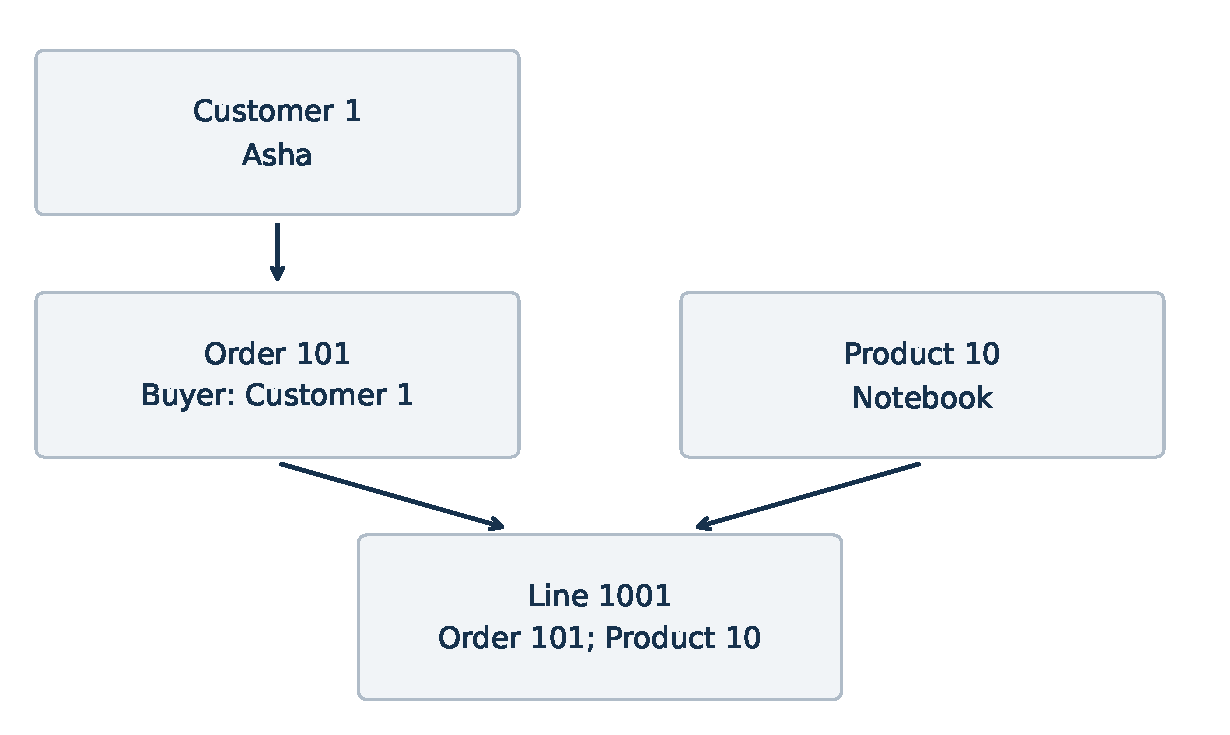
\includegraphics[width=\linewidth]{assets/shop-relationships.pdf}\caption{Required relationships in the teaching example. Arrows run from a parent to its child. To keep Line 1001, the app follows its requirements back to Order 101, Customer 1 and Product 10.}\end{figure}

\section{Set a 50-percent limit}
Half of 13 is 6.5. A database cannot keep half a record, so the allowed row count is rounded down to \textbf{6}. The program counts every kept customer, product, order and line toward that limit.

If the first selected line uses four slots, only two slots remain. The percentage is a maximum, so the application does not promise that exactly half of all original rows will appear.

\section{Add Line 1002}
Line 1002 uses the same Order 101 and Customer 1 that are already selected. Those two records do not need to be copied again. This time only Product 20 and Line 1002 are new.

The first line cost four records. The second line adds two. The copy now contains exactly six records and has reached the limit. This extra cost is called \textbf{incremental cost}: only count records that have not already been selected.

\section{The resulting copy}
\begin{longtable}{>{\RaggedRight\arraybackslash}p{.25\linewidth}>{\RaggedRight\arraybackslash}p{.16\linewidth}>{\RaggedRight\arraybackslash}p{.16\linewidth}>{\RaggedRight\arraybackslash}p{.31\linewidth}}
\toprule\textbf{Table} & \textbf{Original} & \textbf{Copy} & \textbf{Kept IDs}\\\midrule\endhead
Customers & 3 & 1 & 1\\Products & 3 & 2 & 10, 20\\Orders & 3 & 1 & 101\\Order lines & 4 & 2 & 1001, 1002\\\midrule
\textbf{Total} & \textbf{13} & \textbf{6} & All required parents are present.\\\bottomrule
\end{longtable}
There are seven omitted records. An omitted record is not automatically an error: the purpose is to create a smaller copy. A missing \emph{required parent of a retained record} would be an error.

The six-record copy fits the limit and keeps the required parents. We can now ask how useful its query answers remain.

\chapter{From your click to the finished copy}
\section{First see the whole journey}
\begin{figure}[htbp]\centering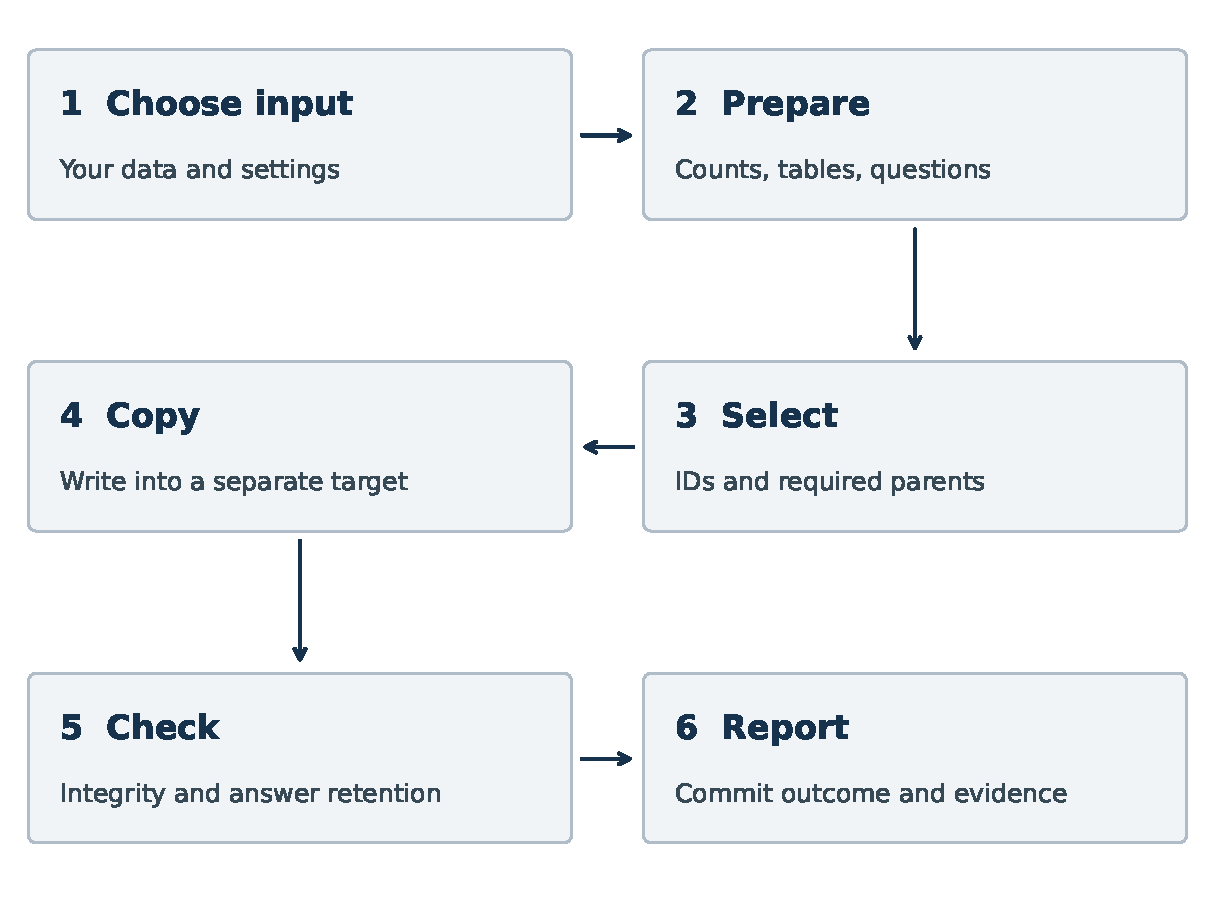
\includegraphics[width=\linewidth]{assets/simple-workflow.pdf}\caption{The user-visible journey. Selection chooses identifiers; copying writes records; checking decides whether that transaction can be accepted.}\end{figure}
This chapter explains each box in the order it occurs. The names in the file guide later describe the same work at code level.

\section{Step 1: read your choices}
\textbf{What goes in?} The selected input, copy percentage, method, seed and any custom SQL workload.

\textbf{What happens?} The app checks that the choices are usable. For example, the percentage must be between 1 and 100 in the desktop app. If a workload file was chosen, that file must exist. Invalid choices should fail before the program prepares new data.

\textbf{What comes out?} A request object. Think of it as the completed instruction form for the job. In the shop illustration, the important entries are a 13-row source, a 50-percent limit and the chosen test questions.

\textbf{Where is this done?} The window is in \path{desktop.py}; request checking and service coordination are in \path{desktop_service.py}. Terminal commands enter through \path{cli.py}.

\section{Step 2: preview and prepare the input}
The preview reads enough of the input to report its row and column counts and find problems. For files, it uses the same table reader as the import path, which helps keep preview and actual import consistent.

For an \textbf{existing MySQL database}, the app reads the source using the configured source connection. It prepares a separate target. For a \textbf{CSV or Excel file}, it first creates a newly owned source database on the configured target server, imports the file there, and prepares a second database for the smaller output.

The imported file values are text. A string such as 0012 should remain 0012. The app adds a record identifier but cannot discover true business relationships just from columns whose names look related. Choose an already structured MySQL database when your test needs real declared foreign keys.

\section{Step 3: describe the tables and their connections}
The program discovers table names, columns, declared primary keys, foreign keys and row counts. The technical name for this table blueprint is the \textbf{schema}.

It also builds a \textbf{dependency graph}, which is a map of which tables depend on which parents. In the shop, order lines need Orders and Products; Orders need Customers. The map helps calculate required parents and determine a safe copying order.

Every supported table needs a declared primary key. Cross-table cycles, composite foreign keys and certain other structures are outside this version's supported scope. A clear unsupported-input message is more useful than a copy the application cannot verify properly.

A cross-table cycle occurs when dependencies loop through tables, such as A requiring B and B requiring A. A composite foreign key is one relationship using several columns together; this version can handle a composite primary key but not that composite relationship. A self-reference stays inside one table, such as an employee referring to a manager. It is supported when following the actual parent records does not form a loop.

\section{Step 4: keep a consistent source view}
Suppose somebody changes an order while a copy is being made. Comparing an old selected row with a newer source answer could be confusing. The normal pipeline therefore keeps selection, copying and query comparison on the same source read view.

The program also records a compact check value based on structure and record values. This is called a \textbf{fingerprint}. It can detect changed values even if the number of rows stayed the same. The fingerprint is evidence about the observed source view; it is not a log proving that no external writer ever made a change.

The related files are \path{connection_scope.py} and \path{source_snapshot.py}. You can understand their purpose first as ``use one consistent original and record what was observed''.

\section{Step 5: read the questions we will test}
The app reads the workload file, separates its statements and assigns query numbers. It understands only the supported SQL patterns. Unsupported statements are reported with a reason so a reader can tell which questions were actually evaluated.

A supported query can also fail when executed, for example because it names an absent column. That is an execution failure, which must remain visible in results. It should not quietly disappear from the comparison as if it had never been requested.

The parser-related files are \path{sql_lexer.py} and \path{workload_analyzer.py}. The next chapter explains how the questions can influence record selection.

\section{Step 6: choose IDs and required parents}
The selector chooses identifiers rather than immediately copying full rows. Whenever it considers a child, it finds the required parent records and checks how many new slots would be used.

For our first sale line, the answer is four. For our second line, the answer is two. If a candidate needs more new records than the remaining space, it cannot be accepted. The selector may finish below the limit if no remaining candidate fits.

The selected-ID result is handed to the copying code. At this moment, a selection exists, but it is too early to call the output a ready, committed copy.

\section{Step 7: copy the records in a safe order}
Customers and Products are copied before dependent records that reference them. Orders are copied before their lines. This keeps the inserts consistent with the relationship rules.

When replacing an existing compatible test target, the old rows are removed in the reverse dependency direction: children before parents. The project also handles supported self-referencing rows in an order where their parent rows come first.

The app compares each inserted batch back to its original values. It also checks the actual target row count rather than assuming every write did what was intended. \path{subset_generator.py} owns this copying work.

\section{Step 8: check before saving the transaction}
A \textbf{transaction} groups related database changes. A \textbf{commit} makes those changes permanent. A \textbf{rollback} cancels the pending changes. Think of this as the database's way to accept or reject a set of related edits together.

Before committing the copied rows, SafeSliceSQL runs the chosen questions, checks the structure and applies the requested quality limits. If these checks reject the copy, the target's pending row changes are rolled back. That protects an earlier valid target's rows from an unacceptable replacement.

There is an important MySQL boundary: creating or removing table structures is not protected in exactly the same way as ordinary row changes. The program attempts scoped cleanup on handled failures, but a hard crash can leave empty table or schema remnants. Keep test targets separate from valuable existing data.

\section{Step 9: show results and record what happened}
A successful result includes the actual copied row count, validation results, query results and timings. A failed attempt should include its reason. The app saves structured files so the result can be inspected after the window closes.

\textbf{Verify my copy} can inspect copied records beside their originals and follow relationships. \textbf{Verify again} reads current contents; it is a new inspection. A saved report describes the recorded time and should be introduced as saved evidence in a presentation.

\section{Who coordinates all these steps?}
\path{pipeline.py} contains the main single-run coordinator, \path{run_pipeline()}. It calls the relevant specialists and collects their results. \path{sampler.py} is the main selection algorithm file. \path{desktop.py} and \path{cli.py} are the entry points used to start work.

These are different meanings of ``main''. A project can have an interface entry point, an algorithm owner and a workflow coordinator without one file doing every job.

\chapter{How the three methods choose records}
\section{What all three methods share}
All methods must obey the same row budget and supported relationship rules. They eventually use the same copying and checking machinery. Their main difference is the order and priorities used to consider candidate records.

That shared machinery matters for a comparison. If one method ignored parent costs or used a different validator, a higher score would be difficult to interpret fairly.

\section{Random-repair: try shuffled candidates}
Imagine a shuffled list of possible records. The method considers a record, finds the parents it needs and checks whether the full new set fits. It accepts feasible additions and continues through candidates.

``Repair'' here means adding needed parents while checking the budget. The method does not simply keep six unrelated children and then add unlimited parents afterward. In the shop, a shuffled candidate line may require four slots even though it is only one sale line.

Random-repair is a useful baseline: it shows how a method can behave without deliberately prioritizing the declared questions.

\section{Referential: work through the relationship order}
This method visits parent tables before dependent tables and makes seeded random choices within that structure. In the shop, it considers parent information before reaching line records.

The approach can produce valid relationships, but the budget may be spent on parent records before enough child records are kept to answer a particular question. This is why structural order alone does not guarantee the most useful copy.

\section{Workload-aware: consider the chosen questions}
Suppose Q1 asks about notebook sales. The workload-aware method first looks for actual records that satisfy the relevant filters and joins. A matching notebook sale is a more direct starting point for that question than an arbitrary unrelated product.

A small set of records demonstrating that a query's conditions can match is called a \textbf{witness}. For a joined sale query, the witness may include identifiers from more than one participating table. Its missing parents still count toward the budget.

The method gives different usable queries a turn rather than letting the first query consume all witness opportunities immediately. Queries explicitly marked required receive priority within those rounds. Remaining space is filled using table priorities derived from workload features.

\section{What are the priority numbers?}
The code uses fixed additions to a table's priority. Each reference in a usable query contributes 2.0. A detected filter column contributes 1.0 to its table. Each resolved grouping column contributes 1.5. The first table in a query also receives 0.5 per detected join pair and an extra 1.0 when the query groups or aggregates. A table receiving no contribution uses a default priority of 1.0.

These values are \textbf{design choices in a heuristic}. They were not learned by training an AI model. ``Heuristic'' means a practical rule for making useful choices without proving it is the best possible solution for every input.

For example, a one-table query with one recognized filter and no grouping contributes $2+1=3$. This score helps decide priority; the record's required parents must still fit. A high priority does not allow the method to exceed the budget.

Now consider only our notebook-sale question Q1. It references Order lines and Products, giving each 2.0. It contains one detected join pair, adding 0.5 to the first table, Order lines. Its product-name filter adds 1.0 to Products. For this one question, their priorities are therefore 2.5 and 3.0. Orders and Customers remain at their fallback priority of 1.0 if no other question weights them.

Those numbers do not mean that Orders and Customers can be discarded. They are required by a retained sale line regardless of table priority. The query witness finds a real notebook sale, and dependency closure brings in its needed order and customer. Scores help organize choices; relationships determine which extra records a choice must carry. When several workload questions are used, their contributions accumulate.

\section{Why not inspect every possible combination?}
Even a modest database can have an enormous number of possible subsets. Trying every possible combination would quickly become impractical. The implementation considers a bounded candidate pool and uses seeded sampling and practical priorities.

The candidate pool aims at about 1.25 times the requested row budget, capped by source size, with per-table rounding rules. For suitable dense integer identifiers, the code can try indexed guesses. Other cases stream an ordered list of keys and keep a seeded sample.

This saves some selection memory and work. It does not mean the entire operation reads only the final copied rows: source fingerprinting and some sampling paths still scan the original data.

\section{What does seed 42 do?}
A \textbf{seed} starts the pseudo-random choices in a repeatable way. With unchanged input, code, workload and compatible execution conditions, using the same seed allows the selection to be repeated. It is useful for reproducing an experiment or comparing methods under consistent settings.

Seed 42 is a default, not a quality score. Seed 999 is not automatically better than seed 42. To compare methods, use a set of seeds and report what actually happened across those trials.

\section{Will workload-aware always be best?}
No universal winner is guaranteed. A heuristic's priorities may help one workload and spend budget less effectively for another. Shared parents, skewed data, very small budgets and grouping requirements can all matter.

The saved World experiment in this project actually shows random-repair ahead of workload-aware on some reported averages. That is a valid experimental outcome. A good project review explains the evidence rather than assuming the proposed method must win.

\reviewpoint{The contribution is a checked way to prioritize real query witnesses and workload-related records under a hard dependency-aware budget. It is not a proof that the smallest or best possible subset has been found.}

\chapter{Read the percentages without getting misled}
\section{Start with the question each number answers}
Results can show several percentages. They measure different things. Before reading a number, ask what is being counted: database records, queries, query-answer rows or groups of answers.

\begin{figure}[htbp]\centering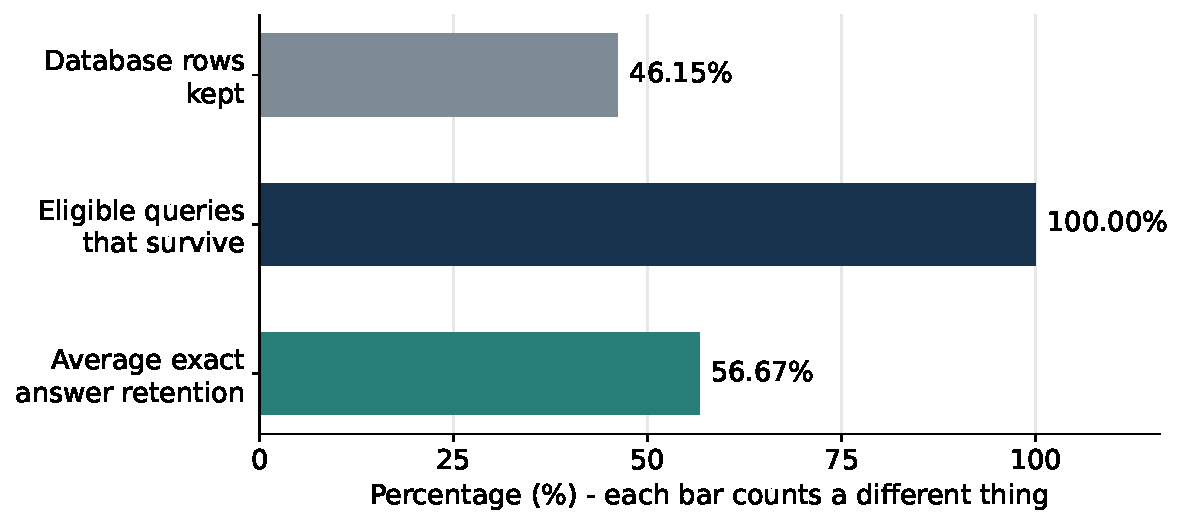
\includegraphics[width=\linewidth]{assets/three-percentages.pdf}\caption{Three different measures from the executed teaching example. They use different denominators, so their values can differ without contradicting each other.}\end{figure}

\section{Physical record retention: how much data was copied?}
The original shop has 13 records across its four tables. The copy has 6. Therefore $6/13\times100=46.15\%$ of its database rows were kept.

The requested limit was 50 percent, but rounding half of 13 down to six gives an actual retained fraction of 46.15 percent. The copy respects the maximum. This percentage says how much data was retained, not how many query answers remain.

\section{Query survival: does a question still return results?}
A query survives when it returns at least one result row on both the source and the target. A known source-empty query is omitted from the survival denominator, because a question with no original matches cannot demonstrate preserved nonempty answers.

In our five-question workload, four queries have nonempty source results. All four also have nonempty target results, so query survival is $4/4=100\%$. The deliberately empty fifth query is handled separately.

Survival is an initial usefulness check. The next examples show why you still need to inspect the actual answer rows.

\section{Q1: ask for notebook sale details}
\begin{lstlisting}[language=SQL]
SELECT l.line_id, p.product_name, l.quantity
FROM order_lines l
JOIN products p ON l.product_id = p.product_id
WHERE p.product_name = 'Notebook';
\end{lstlisting}
There is one matching line in the original: Line 1001, Notebook, quantity 2. That identical result also appears in our copy. The query survives and keeps 1 of 1 original answer rows, or 100 percent.

Notice that the question uses both Order lines and Products. Keeping a line with a missing Product 10 would break the relationship needed to display Notebook. That is why the parent record was copied too.

\section{Q2: ask for every sale-line record}
\begin{lstlisting}[language=SQL]
SELECT line_id, order_id, product_id, quantity
FROM order_lines;
\end{lstlisting}
The original returns four answer rows, one for each sale line. The copy returns two, and both match their original values. The query survives because it still returns results. Its \textbf{exact result-row retention} is $2/4=50\%$.

``Exact'' means the compared answer tuple has the same values in the same output positions. The result comparison also respects duplicate multiplicities. If the original contains a particular output tuple twice and the copy returns it once, only one of those two occurrences has been retained.

\section{Q3: count sale lines by product}
\begin{lstlisting}[language=SQL]
SELECT p.product_id, COUNT(*) AS line_count
FROM products p
JOIN order_lines l ON p.product_id = l.product_id
GROUP BY p.product_id;
\end{lstlisting}
Here the answer contains one row per product group, not one row per sale line:
\begin{longtable}{>{\RaggedRight\arraybackslash}p{.27\linewidth}>{\RaggedRight\arraybackslash}p{.29\linewidth}>{\RaggedRight\arraybackslash}p{.32\linewidth}}
\toprule\textbf{Product group} & \textbf{Original line count} & \textbf{Copy line count}\\\midrule\endhead
10: Notebook & 1 & 1\\20: Pen & 2 & 1\\30: Bag & 1 & Absent\\\bottomrule
\end{longtable}
Two of the three original product groups remain, so \textbf{group coverage} is $2/3=66.67\%$. The pen group remains, but its count changed. Only the complete Notebook answer row is exactly unchanged, so exact result-row retention for this query is $1/3=33.33\%$.

The project calls this group-coverage measure \textbf{aggregate retention} when the grouping keys can be mapped safely to the output. It is useful for understanding which groups survived. It is not a measure of how close each numeric total is to the original total.

The same direction explains a business-rule limit. A retained order need not keep every original line. An invoice's stored total can therefore differ from the sum of its retained lines. Extra business rules may need additional workload checks or another validation design, even when all declared parent relationships are valid.

\section{Q4: count all sale lines}
\begin{lstlisting}[language=SQL]
SELECT COUNT(*) AS total_lines FROM order_lines;
\end{lstlisting}
The original returns one answer row containing the number 4. The copy returns one answer row containing the number 2. Each query result has one row, so the query survives.

However, the answer row containing 4 is different from the answer row containing 2. None of the original complete answer row was retained exactly, so its exact retention is 0 percent.

This also explains an easy trap: COUNT can return one result row containing zero when the underlying table is empty. A surviving count query does not, by itself, prove the copied table contains records.

\section{Q5: ask about an absent customer}
\begin{lstlisting}[language=SQL]
SELECT customer_id, customer_name
FROM customers WHERE customer_id = 999;
\end{lstlisting}
Customer 999 exists in neither database. Both results are empty. The project assigns matching empty/empty results retention 1.0, meaning 100 percent for this comparison. It does not mark the query as surviving, and it excludes this known source-empty query from the survival denominator.

These conventions must be stated because they influence averages. A workload full of empty queries would not be strong evidence that a copy remains useful.

\section{Put the five query results together}
\begin{longtable}{>{\RaggedRight\arraybackslash}p{.12\linewidth}>{\RaggedRight\arraybackslash}p{.27\linewidth}>{\RaggedRight\arraybackslash}p{.23\linewidth}>{\RaggedRight\arraybackslash}p{.26\linewidth}}
\toprule\textbf{Query} & \textbf{Answer rows: source/copy} & \textbf{Survives?} & \textbf{Exact retention}\\\midrule\endhead
Q1 & 1 / 1 & Yes & 100.00\%\\
Q2 & 4 / 2 & Yes & 50.00\%\\
Q3 & 3 / 2 & Yes & 33.33\%\\
Q4 & 1 / 1 & Yes & 0.00\%\\
Q5 & 0 / 0 & Source-empty & 100.00\%\\\bottomrule
\end{longtable}
The average exact retention adds the five query fractions and divides by five:
\[
\frac{1+0.5+\tfrac13+0+1}{5}=0.5667=56.67\%.
\]
The project averages supported queries equally. It does not multiply a query's weight by the number of answer rows it originally returned. Our 56.67 percent is therefore different from the 46.15 percent of physical database rows kept.

\section{What does key retention mean?}
An identifier tells you which record an answer concerns. \textbf{Key retention} checks how many distinct original identifiable keys remain in the target's answers when the program can map those keys reliably.

For Q2, the copied line IDs are 1001 and 1002 out of four original line IDs, so key retention is 50 percent. For Q3, product IDs 10 and 20 remain out of three original product IDs, so it is 66.67 percent even though one group's count changed. The checked example's average key retention is 63.33 percent.

When the output does not provide a safely recognized key, the evaluator uses exact result-row retention as its fallback. A column merely being named something ending in ``id'' is not sufficient proof that it is the correct record identifier.

\section{Read integrity results before celebrating a percentage}
\begin{description}[style=nextline,leftmargin=1.5em,labelindent=0pt]
\item[Duplicate primary keys] Two copied records share the same declared identifier tuple. A valid copy must not have this problem.
\item[Foreign-key violations] A retained non-null child reference has no matching parent. The required count is zero.
\item[Actual rows versus budget] The program counts rows actually present in the target, including all copied tables. In the example this is 6 versus a limit of 6.
\item[Schema compatibility] The table definitions and supported constraints agree with the original. A table with the right name but the wrong rules is insufficient.
\item[Copied values] Retained records match their original values. A missing deliberately unselected record is different from a changed copied value.
\item[Source unchanged] This can be verified True, detected False or unverified. A later validation without an earlier content baseline cannot reconstruct the source's past state.
\end{description}

\section{What if a query fails or is unsupported?}
An unsupported SQL form is excluded with a reason. It should remain visible so you can see that the project did not measure that question. A supported query that fails during execution remains a failure and contributes zero retention; it should not quietly improve the reported average by disappearing.

If source execution fails and no successful earlier evaluation proves the source result empty, that query is conservatively treated as an eligible survival failure. These rules protect the meaning of the percentages.

\reviewpoint{A useful sentence for your review is: ``I check relationship validity first, then whether queries still produce results, then how many original answers remain exactly. Each number answers a different question.''}

\chapter{Understand the settings}
\section{The settings you will use most}
\begin{description}[style=nextline,leftmargin=1.5em,labelindent=0pt]
\item[Input] Choose one existing MySQL database, one CSV, a folder of CSVs or an XLSX workbook. A downloaded SQL dump must first be loaded using a MySQL client.
\item[Budget percentage] The maximum total number of source records the copy may keep. It includes parents. For 13 source records and 50 percent, the cap is 6.
\item[Method] The strategy for choosing candidates: random-repair, referential or workload-aware. The desktop default is workload-aware.
\item[Seed] A repeatability setting; the default is 42. Keep it the same when reproducing a run.
\item[Workload file] The questions to evaluate. For a meaningful business test, choose questions matching that database and scenario.
\item[Compare methods] Runs multiple experiments rather than creating a merged copy. Each experiment refreshes the target. The target afterward reflects the last successful committed run.
\end{description}

\section{Two quality limits that are easy to confuse}
\textbf{Minimum query survival} requires enough eligible questions to still return results. The desktop default is 100 percent. A query that returns a different numeric total can still survive, as Q4 showed.

\textbf{Minimum exact result retention} requires the average exact answer preservation to reach a chosen fraction. The default is zero, so survival and structural checks can be accepted even when exact retention is low.

In the shop example, a survival threshold of 100 percent passes. An exact-retention threshold of 60 percent fails, because the measured average is 56.67 percent. The quality gate should reject that attempt before the row transaction commits. This explains why a copy can be structurally sound yet unacceptable for a chosen workload requirement.

CLI and library defaults keep both minimum thresholds at zero for compatibility; a review experiment should state the chosen thresholds explicitly. Internal settings use fractions such as 0.6; the desktop presents user-facing percentages.

\section{Required query IDs}
If Q1 is critical, you can require Q1 to survive. The query must exist, be supported, execute successfully and return a surviving result. A required query that is absent, excluded, failed or lost rejects the copy.

Query IDs follow statement order in the workload file. Reordering statements can therefore change which question ``Q1'' means. Review your required IDs after editing the workload.

\section{Resource limits are stop rules}
The default whole-job time limit is 600 seconds, the statement setting is 30 seconds and the connection limit is 10 seconds. The public configuration also limits source rows, streamed query rows, input size, temporary comparison space, client memory, tables and columns.

These settings help stop unexpectedly large work. They do not prove that the application has successfully processed every permitted size. For example, a default maximum of 5,000,000 source rows is a guard value; it is not a benchmark certificate for five million rows.

Cancellation and some resource checks happen at safe checkpoints. They are cooperative controls rather than hard operating-system resource isolation. Keep a cancelled job open until it returns, and inspect whether a commit had already completed.

\section{The most useful function inputs and outputs}
\begin{longtable}{>{\RaggedRight\arraybackslash}p{.28\linewidth}>{\RaggedRight\arraybackslash}p{.30\linewidth}>{\RaggedRight\arraybackslash}p{.30\linewidth}}
\toprule\textbf{Operation} & \textbf{Information received} & \textbf{Information returned}\\\midrule\endhead
Describe the source & A connection to the source & Tables, keys, relationships and counts\\[4pt]
Choose records & Description, method, budget, seed, workload & Selected record IDs and selection diagnostics\\[4pt]
Copy selected records & Source, target and selected IDs & Copy success/failure and inserted counts\\[4pt]
Evaluate questions & Source, target and workload & Each query's counts, retention and errors\\[4pt]
Validate the copy & Source, target and row cap & Structural checks and source evidence\\[4pt]
Coordinate one run & All prepared inputs and quality settings & One complete run result, with timings and errors\\\bottomrule
\end{longtable}
Their code names are \path{inspect_schema()}, \path{select_rows()}, \path{materialize_subset()}, \path{evaluate_workload()}, \path{validate_subset()} and \path{run_pipeline()}. The technical companion gives their complete signatures. This guide first explains why those inputs and outputs exist.

\chapter{Run your first real test}
\section{Start with a simple successful run}
Open PowerShell in the project folder and launch the app:
\begin{lstlisting}[language={}]
cd C:\Users\saivi\Projects\SafeSliceSQL
.\demo.bat
\end{lstlisting}
A Python virtual environment, installed requirements and working MySQL connection must already be configured. The README contains installation steps. If the desktop does not open, use the console interpreter to display the error:
\begin{lstlisting}[language={}]
.\.venv\Scripts\python.exe -m safeslicesql.desktop
\end{lstlisting}
For the tiny bundled demo, choose \path{examples/demo-orders.csv}, set 25 percent and create the copy. Twenty source rows permit five target rows. Use this to learn the controls; it is deliberately below the larger-input testing threshold.

\section{Then use a source above 5,000 rows}
\begin{longtable}{>{\RaggedRight\arraybackslash}p{.23\linewidth}>{\RaggedRight\arraybackslash}p{.20\linewidth}>{\RaggedRight\arraybackslash}p{.45\linewidth}}
\toprule\textbf{Input} & \textbf{Source rows} & \textbf{A useful first purpose}\\\midrule\endhead
World & 5,302 & Follow a city to its country; understand a small relational schema.\\[4pt]
Chinook & 15,607 & Follow invoice lines through invoices, customers and tracks.\\[4pt]
Employees & 3,919,015 & Explore salary history and larger scans after smaller runs are comfortable.\\[4pt]
Diamonds CSV & 53,940 & Test a larger single-table import with clear categories.\\[4pt]
Taxis CSV & 6,433 & Test timestamp-like strings, payment categories and empty fields.\\\bottomrule
\end{longtable}
For a database, the count is the total across its base tables. Small lookup tables are normal. The smaller copy may have fewer than 5,000 rows because the minimum concerns the input selected for testing.

Use the README download links and confirm the actual preview count. Local Diamonds and Employees payloads already exist in this checkout. Downloaded payload folders are ignored by Git, so they may be absent in a fresh clone.

\section{Choose the workload that belongs to that input}
For Diamonds imported alone as diamonds.csv, choose \path{workloads/testing_diamonds.sql}. Its queries assume the imported table name \path{data_1_diamonds}. A renamed file or folder import can produce different table numbering, so use the table names recorded in the import manifest.

For World, Chinook and Employees, use their respective testing\_*.sql files. The original \path{workloads/workload.sql} contains Employees questions. Reusing it against an unrelated schema will not turn those questions into suitable queries for that database.

The shop setup and five-question workload from this guide are included under assets. The setup script should be used only in a fresh empty database. The checked six-row copy was deliberately chosen for explanation; it is not a guarantee of what an automatic method will choose for every run.

\section{What should you look at on Results?}
First find whether the run was accepted and the actual target database name. Then compare copied rows with the allowed limit. Inspect validation checks, query errors and exclusions, survival and exact retention.

Open a retained record beside its original, then follow one declared parent. An absent unselected record is expected; a missing required parent is not. Export a report after a successful inspection so you can discuss the exact run later.

\section{Why a standalone validation needs the right cap}
When checking a World copy created at 20 percent, the intended limit is 1,060 rows. Supply that limit explicitly when validating the named source and target from the terminal:
\begin{lstlisting}[language={}]
safeslice validate --source world --target YOUR_COPY_NAME --budget-limit 1060 --workload workloads/testing_world.sql
\end{lstlisting}
Without an explicit cap, standalone CLI validation defaults to the current full source size. That would not prove that a 20-percent limit was respected. Standalone validation also lacks the earlier content snapshot needed to prove what the source looked like at creation time.

\chapter{Read the saved results}
\section{What is actually saved?}
The output database and the report folder are different things. The database stores records. Report files store observations and settings: selected method, budget, seed, row counts, query measurements, validation outcomes and errors.

\begin{description}[style=nextline,leftmargin=1.5em,labelindent=0pt]
\item[dataset.json] Describes the prepared input, table mappings and import semantics.
\item[run.yaml] Records experiment choices such as methods, percentages, seeds, workload and output folders.
\item[job.json] Tracks the job's owner, process, phases, limits, states and newly created schema ownership.
\item[Run and query CSVs] Preserve measured values for one attempt and its individual questions, including failure information.
\item[Combined raw CSV] Lists all experiment attempts; useful for checking successes and failures before averages.
\item[Summary CSV/Markdown and charts] Present grouped measurements across runs. The input records and observation counts still matter.
\item[\path{copy_summary.json} and verification] Describe a saved copy outcome and any recorded inspection. A later database edit can make a fresh inspection differ.
\end{description}

\section{A benchmark means repeated comparable experiments}
A \textbf{benchmark} is a planned comparison. For example, three methods, three budget percentages and two seeds produce $3\times3\times2=18$ runs.

Keep the source, workload and evaluation rules consistent. Otherwise a faster or higher-scoring run might reflect a different task. The project uses the same core pipeline and one shared source read view for a benchmark matrix.

The target is refreshed per run. After the comparison, it contains the last successful committed copy, not every method's records combined. Read the individual report rows to discuss a particular method and seed.

\section{What do mean and standard deviation tell me?}
The \textbf{mean} is the arithmetic average of measured values. If two successful runs take 2 and 4 seconds, their mean is 3 seconds. It does not say that either run actually took exactly 3 seconds.

The \textbf{sample standard deviation} describes how spread out repeated observed values are. The project reports no sample standard deviation when there is only one successful observation. A blank value here is more honest than implying a measured spread of zero.

Failed attempts remain in raw records and failure counts, but performance averages use successful measured runs. Read both the average and the attempted/successful/failed counts. A method that succeeded once out of many attempts should not be presented as reliable simply because that one attempt was fast.

\section{The saved tiny demo teaches an important lesson}
One saved demo copied 5 of 20 records at a 25-percent budget. Its three eligible queries all returned results, so survival was 100 percent. Its per-query exact retention values were 25 percent, zero and 25 percent, giving an average of 16.67 percent.

The count query returned one result row on both sides, but its count changed from 20 to 5. This is the same lesson as our shop Q4. These are saved observations, not an additional freshly rerun MySQL demo for this rewrite.

\section{The older World comparison does not prove a universal winner}
The saved World experiment has 18 runs over 5,302 source rows. At a 10-percent budget, recorded means include 100-percent survival and 15.03-percent exact retention for random-repair, compared with 83.33-percent survival and 12.60-percent exact retention for workload-aware.

The artifact date is 2 November 2026, earlier than the inspected source snapshot. It has no embedded source commit and uses older recorded timing fields. It describes those saved runs; it does not establish performance of every current method revision or future dataset.

A useful project review can say: ``The method comparison is empirical. In this saved example the baseline did better, so I do not claim workload-aware always wins. I would rerun the current code with more seeds and a representative workload before making a general claim.''

\section{What do the saved scale checks establish?}
One recorded MySQL synthetic sweep tested five schema shapes and all three methods at 10- and 100-percent budgets. Each scale sample contained 30 checks with zero recorded failures. The largest case in the larger sample had 40,463 total source rows.

That larger sample recorded about 426.58 seconds of wall time and 262.73 MiB sampled peak client memory. This is evidence from a generated-data test. It does not measure the MySQL server's total resources or certify production capacity.

The generated row setting is a bound per table. A request for 10,000 rows in that generator can produce more than 10,000 total rows across several tables. Always read the actual case totals rather than presenting the generator setting as the whole database size.

\chapter{Explain the project in your review}
\section{A simple opening explanation}
You can begin with the following explanation in your own words:

``SafeSliceSQL helps create a smaller working copy of a relational database. The difficult part is that records depend on other records. If I keep a sale, I may also need its order, customer and product. My project includes those required parents within the same row limit, then checks the copy and measures what happens to a chosen list of SQL questions.''

This opening gives the problem, the dependency rule and the measured outcome before naming algorithms or modules.

\section{Show one record's full journey}
Use Line 1001 from the teaching example. Show its parent requirements, count the four required records and add Line 1002 for two more slots. Then show the copied table counts and one query whose answer changed.

This makes the budget and dependency logic visible. It is easier to follow than reading every method signature aloud. Once the example is understood, point to the code files responsible for the same stages.

\section{The files to highlight first}
\begin{enumerate}
\item \path{pipeline.py}: connects the complete single-run process and checks before commit.
\item \path{sampler.py}: implements the three record-selection strategies.
\item \path{dependency_graph.py}: finds required parents and incremental closure.
\item \path{subset_generator.py}: writes selected records in a safe order and compares copied values.
\item \path{validator.py}: checks integrity and evaluates the declared workload.
\item \path{desktop.py} and \path{cli.py}: let a user run the same underlying work through different interfaces.
\end{enumerate}
After that, use the next chapter's file guide to explain supporting responsibilities without pretending every file is an independent algorithm.

\section{Questions you should be able to answer}
\textbf{Why not keep random rows independently?} Because a retained child can reference a parent that was discarded. Required parents must be included and counted.

\textbf{Does a valid relationship guarantee the same business answer?} No. Many child rows can be omitted while relationships remain valid. The workload measures the resulting answer retention.

\textbf{What does 100-percent survival mean?} Every eligible question still returns at least one row. It does not mean every original answer remains or every count is unchanged.

\textbf{What is the proposed method?} A workload-aware heuristic that first considers actual query witnesses and then fills space using table priorities, always checking missing-parent costs.

\textbf{What happens if a quality limit fails?} The pending target row changes are rejected before commit. Inspect the error and run again with appropriate settings rather than calling the failed attempt ready.

\textbf{What is supported?} MySQL 8.x/InnoDB application inputs, declared primary keys, supported single-column foreign keys and acyclic dependencies, plus the restricted read-only workload subset. File imports preserve text and add IDs.

\textbf{How did you test it?} Explain current non-database tests, generated-schema checks and recorded MySQL evidence separately. State the backend, counts, date, workload and limits of each result you show.

\section{A short presentation order}
\begin{enumerate}
\item Explain the problem using the shop's sale and its parents.
\item Show a real input preview and the chosen row cap.
\item Run or show a clearly labelled saved slice with fixed settings.
\item Show the actual row count, zero missing parents and one kept record beside its original.
\item Explain survival and exact retention using one changed count result.
\item Show one method comparison, including failure counts and evidence boundaries.
\item Finish with supported scope and the next experiment you would run.
\end{enumerate}

\reviewpoint{The strongest review shows that you understand the tradeoff: a small, structurally valid copy can still lose useful answers. The project measures that loss and can reject a copy that falls below explicit requirements.}

\clearpage
\part*{Follow the files without getting lost}
\addcontentsline{toc}{part}{Follow the files without getting lost}
\chapter{How the files work together}

Each file below is explained through a real handoff. Read the job first, then what arrives, what changes and what leaves. The example connects it to the shop. Function names are signposts for later code reading, not terms to memorize before understanding the role.

All paths in this chapter start inside src/safeslicesql/. The separate technical companion contains exact signatures, helper methods, defaults and source line references.

\section{Start a run and read its settings}

\Needspace{11\baselineskip}

\subsection{desktop.py}

\textbf{Its job:} The window you interact with.

\textbf{What arrives.} Your clicks, selected input, percentage, method and other settings.

\textbf{What it does.} It builds the screens, requests an input preview, starts a background copy job and updates the visible progress. A background job lets the window remain usable while database work runs. The window also offers history, verification and result actions.

\textbf{What leaves.} A checked instruction request passed to the desktop service, followed by a visible result or actionable error.

\textbf{Connect it to the example.} You choose the shop database and a 50-percent cap. This file collects those choices; it does not independently decide which sale lines should be kept.

\textbf{Where the work goes next.} It calls \path{desktop_service} for the copy and \path{result_views} for result windows. main() is the desktop start point.

\textbf{Names to find in the code.} Desktop.\_run() starts the user-request flow; Desktop.\_poll() brings worker messages back to the interface.

\Needspace{11\baselineskip}

\subsection{desktop\_service.py}

\textbf{Its job:} Turn window choices into an experiment.

\textbf{What arrives.} The request form, connection configuration, a new report folder and a progress callback.

\textbf{What it does.} It validates the request, prepares input and a separate target, writes experiment settings, opens connections and calls the shared benchmark runner. Even a desktop run with one selected method uses that common runner. Connections are closed when the operation ends.

\textbf{What leaves.} A CopyOutcome containing the request, prepared input, run results and output folder.

\textbf{Connect it to the example.} The shop request becomes a concrete job with a six-row budget, a workload path and a target name. A successful-looking screen still depends on the returned checks.

\textbf{Where the work goes next.} It joins \path{dataset_input}, \path{experiment_config}, benchmark and \path{saved_results} under runtime and job-journal controls.

\textbf{Names to find in the code.} \path{create_copy()} establishes the job lifecycle; \_\path{create_copy()} performs the preparation and run.

\Needspace{11\baselineskip}

\subsection{cli.py}

\textbf{Its job:} Commands typed in a terminal.

\textbf{What arrives.} Command arguments such as method, percentage, source, target, seed and workload.

\textbf{What it does.} It checks command options, loads settings and starts the requested operation. Commands include inspect, run, validate, benchmark, selftest, scalecheck and job management. A dry run selects records without constructing a target copy.

\textbf{What leaves.} Console explanations, exported reports and a success/failure exit status.

\textbf{Connect it to the example.} A terminal user can ask for a 50-percent shop copy using the same underlying selection and validation code as the window.

\textbf{Where the work goes next.} run() uses the shared pipeline. The terminal is another entrance to the project, not a different sampling implementation.

\textbf{Names to find in the code.} app registers the Typer commands; run() coordinates a normal CLI slice.

\Needspace{11\baselineskip}

\subsection{demo.py}

\textbf{Its job:} The numbered terminal menu.

\textbf{What arrives.} Menu choices and editable demonstration settings.

\textbf{What it does.} It lets a presenter choose actions without retyping long commands. It builds argument lists for the existing CLI, prepares selected input and records comparison choices. Cancelling a selection returns to the menu rather than treating missing input as a dataset.

\textbf{What leaves.} The invoked CLI action and its saved report location, or a clear failed-action result.

\textbf{Connect it to the example.} For a shop demonstration, a presenter changes the size and method in the menu, then invokes a real copy instead of a simulated screen.

\textbf{Where the work goes next.} Terminal Demo.bat starts this route through cli demo. The menu reuses the same application components.

\textbf{Names to find in the code.} \path{interactive_demo()} runs the menu; DemoSettings carries the current choices.

\Needspace{11\baselineskip}

\subsection{commands.py}

\textbf{Its job:} Give terminal actions the same safety wrapper.

\textbf{What arrives.} A CLI operation about to run.

\textbf{What it does.} It surrounds that operation with a job record and resource-limit context. This is called a decorator: a reusable wrapper around a function. It also translates cancellation and limit stops into consistent terminal exit codes.

\textbf{What leaves.} A bounded, journaled command result or an explicit stopped/failed exit.

\textbf{Connect it to the example.} A shop command that reaches a configured time limit should stop through the normal cleanup path, rather than continue silently.

\textbf{Where the work goes next.} It works with runtime for limits and jobs for durable local records.

\textbf{Names to find in the code.} \path{bounded_command()} installs this common lifecycle around decorated CLI actions.

\Needspace{11\baselineskip}

\subsection{\_\_init\_\_.py}

\textbf{Its job:} The package introduction and public shortcuts.

\textbf{What arrives.} A Python import of the safeslicesql package.

\textbf{What it does.} It declares the package version and exposes selected library operations through one package name. Re-exporting a function is like making a useful operation available from the package front door; the actual implementation remains in its owning module.

\textbf{What leaves.} Version information and public references to operations such as schema inspection, selection and validation.

\textbf{Connect it to the example.} A Python script may import \path{select_rows} from safeslicesql instead of naming the deeper module path.

\textbf{Where the work goes next.} It connects public names to config, schema, graph, sampler, copying and validation modules.

\textbf{Names to find in the code.} \_\_all\_\_ lists public exports; \_\_version\_\_ records version 0.1.0.

\Needspace{11\baselineskip}

\subsection{config.py}

\textbf{Its job:} Read connection and application settings.

\textbf{What arrives.} The environment and the selected environment-file path.

\textbf{What it does.} It constructs separate source and target settings and checks missing or invalid values. A host is the server address, a port identifies the service endpoint, and a database name chooses the schema on that server. Password representation is masked.

\textbf{What leaves.} AppConfig and DatabaseConfig objects: filled settings forms used by later operations.

\textbf{Connect it to the example.} The shop source might be \path{shop_source} and its target \path{shop_slice}. This file keeps those roles distinct before any records are chosen.

\textbf{Where the work goes next.} db uses its connection settings; security resolves configured password references.

\textbf{Names to find in the code.} \path{load_config()} reads settings. DatabaseConfig.url creates the driver connection URL safely.

\Needspace{11\baselineskip}

\subsection{db.py}

\textbf{Its job:} Connect and confirm database identity.

\textbf{What arrives.} Source/target settings or a database URL.

\textbf{What it does.} It creates connection engines, checks reachability and helps safely name tables. An engine manages database connections; it is not the stored data itself. Identity checks use the actual connected database, protecting against different hostnames that reach the same MySQL server.

\textbf{What leaves.} Usable source/target engine handles or a connection/identity error.

\textbf{Connect it to the example.} Before copying the shop, the application must ensure its target is not the very same original database under another label.

\textbf{Where the work goes next.} Schema inspection, selection and copying use these handles to perform database operations.

\textbf{Names to find in the code.} \path{assert_distinct_databases()} refuses source/target identity conflicts; \path{test_connection()} checks reachability.

\Needspace{11\baselineskip}

\subsection{security.py}

\textbf{Its job:} Handle passwords and safe error messages.

\textbf{What arrives.} Configured environment passwords, secret-file references or native OS-vault references.

\textbf{What it does.} It resolves the chosen credential source and registers secrets for redaction. Redaction means removing a sensitive value from a displayed message. Explicit unreadable references fail instead of quietly choosing a different password. Public database errors omit SQL parameters and bound record values.

\textbf{What leaves.} A usable credential for the connection, or a sanitized error.

\textbf{Connect it to the example.} A failed shop login should tell you to check connection settings without printing your password beside the error.

\textbf{Where the work goes next.} config requests credentials; logging and UI error handling use sanitized messages.

\textbf{Names to find in the code.} credential() resolves a password; \path{safe_error()} prepares an error suitable for ordinary display.

\Needspace{11\baselineskip}

\subsection{logging\_config.py}

\textbf{Its job:} Write useful diagnostics.

\textbf{What arrives.} Configured logging level and log folder, plus messages from application stages.

\textbf{What it does.} It sets up console and rotating file logging. A log is a diagnostic history of events; rotation prevents one file from growing forever. A filter removes registered secrets from messages before they are shown or written.

\textbf{What leaves.} Readable progress/error messages and diagnostic log files.

\textbf{Connect it to the example.} If a shop run fails during copying, logs help locate the phase. They do not replace the CSV evidence about which checks passed.

\textbf{Where the work goes next.} Most modules use the project logger. Configuration chooses how much detail is written.

\textbf{Names to find in the code.} \path{setup_logging()} installs handlers and redaction filtering.

\section{Choose and prepare the input}

\Needspace{11\baselineskip}

\subsection{input\_picker.py}

\textbf{Its job:} Help the user choose an input.

\textbf{What arrives.} A request to browse files/folders or discover source databases.

\textbf{What it does.} It opens the appropriate picker or lists usable database names, excluding system schemas. It handles cancellation as cancellation. Choosing a file here does not yet import it or make a copy.

\textbf{What leaves.} The selected file path or database name, or no selection.

\textbf{Connect it to the example.} The shop database name chosen in a menu becomes a source choice for later preparation.

\textbf{Where the work goes next.} The menu and desktop discovery routes use it before preview/preparation.

\textbf{Names to find in the code.} \path{pick_input()} selects a source; \path{available_databases()} returns user-facing database choices.

\Needspace{11\baselineskip}

\subsection{input\_preview.py}

\textbf{Its job:} Show the input size before copying.

\textbf{What arrives.} An input kind and selected path/database name with the needed configuration.

\textbf{What it does.} It reads files without importing them, or inspects a source database read-only. It counts rows/columns, validates widths and limits, and returns warnings. Its budget calculation follows the copy percentage rounding, with zero displayed for empty input.

\textbf{What leaves.} An InputPreview: table names, row/column counts and warnings.

\textbf{Connect it to the example.} It can show 13 shop records and a maximum of six at 50 percent before selection begins.

\textbf{Where the work goes next.} It shares the file reader with \path{dataset_input} so the preview agrees with import behavior.

\textbf{Names to find in the code.} \path{preview_input()} collects statistics; InputPreview.\path{row_budget()} calculates the displayed cap.

\Needspace{11\baselineskip}

\subsection{dataset\_input.py}

\textbf{Its job:} Prepare the original data and a separate target.

\textbf{What arrives.} Exactly one selected existing database or a selected CSV/folder/XLSX path.

\textbf{What it does.} For file inputs it creates a newly owned imported-source schema and adds generated IDs while keeping cell values as text. For an existing database it preserves declared types and relationships. It prepares a new target, records mappings and attempts ownership-scoped cleanup on a handled preparation failure.

\textbf{What leaves.} PreparedDataset containing source/target configurations, table counts, a workload path and dataset.json.

\textbf{Connect it to the example.} A shop CSV does not magically become four related tables. To test our declared parent rules, use the relational schema rather than expect foreign keys to be inferred from file names.

\textbf{Where the work goes next.} It hands a prepared source and target to the desktop service or menu.

\textbf{Names to find in the code.} \path{prepare_dataset()} chooses the preparation route; \path{import_files()} streams supported tables into an empty source.

\Needspace{11\baselineskip}

\subsection{automatic\_workload.py}

\textbf{Its job:} Create basic questions from discovered tables.

\textbf{What arrives.} The source table description, including its keys and relationships.

\textbf{What it does.} It generates structural SELECT questions: list records, count them, group a category and follow a declared relationship. Large example projections are ordered and bounded. It does not infer what matters most to a business from the table names alone.

\textbf{What leaves.} A SQL string or saved automatically named .sql workload file.

\textbf{Connect it to the example.} For a shop it can produce a basic order-to-customer join. A requirement such as notebook-sale coverage should still be expressed in an appropriate custom query.

\textbf{Where the work goes next.} \path{dataset_input} uses it during preparation; CLI/benchmark can request an auto workload too.

\textbf{Names to find in the code.} \path{generate_workload()} builds SQL; \path{save_automatic_workload()} writes it into the report area.

\Needspace{11\baselineskip}

\subsection{experiment\_config.py}

\textbf{Its job:} Write the experiment instruction sheet.

\textbf{What arrives.} Methods, budgets, seeds, workload path, quality thresholds and output folder.

\textbf{What it does.} It writes these choices in YAML, a structured text settings format. Using one writer helps desktop and terminal menu runs describe their experiments consistently. Workload/output paths are resolved so later execution knows which files were intended.

\textbf{What leaves.} A configuration-file path that the benchmark runner can read.

\textbf{Connect it to the example.} The shop settings might say one method, budget 50, seed 42 and the five-question shop-workload.sql file.

\textbf{Where the work goes next.} \path{desktop_service} and demo call it; benchmark consumes its output.

\textbf{Names to find in the code.} \path{write_experiment_config()} creates the YAML instruction file.

\section{Understand the source and choose records}

\Needspace{11\baselineskip}

\subsection{schema\_analyzer.py}

\textbf{Its job:} Discover the table blueprint.

\textbf{What arrives.} A connection to the source, optionally with already verified row counts.

\textbf{What it does.} It asks the database which tables, columns, identifiers and foreign keys are declared. It obtains exact table counts or reuses counts from the same source view. Missing primary keys and unsupported structures are recorded; inspection failures do not become fake zero counts.

\textbf{What leaves.} SchemaMetadata containing a TableMetadata description for each table.

\textbf{Connect it to the example.} It discovers that Order lines has \path{line_id} as its ID and that \path{order_id} and \path{product_id} point to two parents.

\textbf{Where the work goes next.} \path{dependency_graph} turns these descriptions into a dependency map; selection and copying read the same descriptions.

\textbf{Names to find in the code.} \path{inspect_schema()} returns the structured source description.

\Needspace{11\baselineskip}

\subsection{dependency\_graph.py}

\textbf{Its job:} Find everything a record needs.

\textbf{What arrives.} Table/key descriptions, candidate IDs, a source connection and any already selected records.

\textbf{What it does.} It builds the table dependency map and follows real foreign-key values to parent IDs. It keeps following parents until all requirements are covered. Already selected parents are treated as paid for. Nullable references can mean no parent is required; supported unique-column references are resolved to actual parent primary keys.

\textbf{What leaves.} A required-record closure, added-parent information and a safe table order.

\textbf{Connect it to the example.} Line 1001 requires four records. Once those are selected, Line 1002 requires only two new ones. This file supplies that relationship reasoning.

\textbf{Where the work goes next.} sampler asks it for closure; \path{subset_generator} uses its parent-first order.

\textbf{Names to find in the code.} \path{compute_closure()} finds required records. DependencyGraph.\path{topological_order()} gives a valid table order.

\Needspace{11\baselineskip}

\subsection{sql\_lexer.py}

\textbf{Its job:} Recognize SQL text boundaries correctly.

\textbf{What arrives.} The raw text of a workload file.

\textbf{What it does.} It separates words, quoted strings, identifiers, comments and statement terminators. A semicolon inside a quoted value must not split one query into two. Unterminated text and executable comments are rejected rather than guessed at.

\textbf{What leaves.} Tokens or a list of intact SQL statements for further analysis.

\textbf{Connect it to the example.} A shop product name containing punctuation or an apostrophe should remain part of the intended value, not change where a question ends.

\textbf{Where the work goes next.} \path{workload_analyzer} uses it to read queries and interpret features safely within the supported subset.

\textbf{Names to find in the code.} tokenize() recognizes pieces of SQL; \path{split_statements()} produces the statement list.

\Needspace{11\baselineskip}

\subsection{workload\_analyzer.py}

\textbf{Its job:} Understand which questions can be measured.

\textbf{What arrives.} A workload path and optionally a source connection.

\textbf{What it does.} It assigns Q numbers, finds referenced tables, joins, conditions, groups and aggregates, and records whether each SQL pattern is supported. It can stream source counts, although normal pipeline setup postpones those executions to the later comparison stage.

\textbf{What leaves.} WorkloadAnalysis containing QueryInfo records and reasons for exclusions/errors.

\textbf{Connect it to the example.} For the notebook question it recognizes Order lines joined to Products with a product-name filter. That helps later selection find relevant records.

\textbf{Where the work goes next.} sampler reads features and usable-query status; validator executes and compares the questions.

\textbf{Names to find in the code.} \path{analyze_workload()} prepares the query descriptions; \path{require_usable_workload()} rejects an unusable workload.

\Needspace{11\baselineskip}

\subsection{workload\_candidates.py}

\textbf{Its job:} Find real rows matching a question.

\textbf{What arrives.} One supported query, the schema, source connection and a row-witness limit.

\textbf{What it does.} It keeps the original FROM, JOIN and WHERE conditions but projects participating primary keys. This produces a bounded set of actual matching record combinations. It does not solve every group-total or HAVING requirement optimally.

\textbf{What leaves.} Small witness sets of table names and record IDs.

\textbf{Connect it to the example.} For notebook-sale details, a witness can identify the matching sale line and Product 10 instead of simply preferring every product equally.

\textbf{Where the work goes next.} The workload-aware sampler uses these witnesses before filling remaining space with other candidates.

\textbf{Names to find in the code.} \path{query_witnesses()} finds the bounded real matches.

\Needspace{11\baselineskip}

\subsection{sampler.py}

\textbf{Its job:} Choose which record IDs to keep.

\textbf{What arrives.} Schema, dependency map, source, budget, method, seed and any usable workload.

\textbf{What it does.} It dispatches one of the three methods, builds candidate samples, requests required-parent closure and accepts additions only when their new cost fits. Workload-aware selection considers query witnesses and table priorities; the two baselines use different consideration orders.

\textbf{What leaves.} SelectionResult with chosen IDs, total count, added-parent count, rejections and a bounded decision log.

\textbf{Connect it to the example.} It may accept the four-record requirement for Line 1001, then the two-record addition for Line 1002, and stop at six. Our particular IDs are a teaching choice, not a promised automatic selection for every setting.

\textbf{Where the work goes next.} pipeline passes this result to \path{subset_generator}. Selection is a plan for copying, not a committed target.

\textbf{Names to find in the code.} \path{select_rows()} is the main selector interface. Its default library budget is zero and seed is 42.

\section{Copy records and decide whether to accept them}

\Needspace{11\baselineskip}

\subsection{pipeline.py}

\textbf{Its job:} Coordinate one complete checked slice.

\textbf{What arrives.} The prepared source/target connections, schema, graph, workload, cap, method, seed, baseline and quality settings.

\textbf{What it does.} It verifies the source baseline, takes the target lease, invokes selection and copying, and arranges evaluation/validation before commit. It times stages and returns collected evidence when a stage fails. A callback is work scheduled to run at a specific point; here that point is just before the copied-row transaction can commit.

\textbf{What leaves.} One BenchmarkRunResult containing selection, generation, checks, acceptance, timings and error state.

\textbf{Connect it to the example.} A six-row shop plan must still pass value, relationship, budget and query-quality checks before this operation can be called successful.

\textbf{Where the work goes next.} The desktop benchmark runner and CLI both call this coordinator.

\textbf{Names to find in the code.} \path{run_pipeline()} is the best single file entry for understanding how a full run is joined together.

\Needspace{11\baselineskip}

\subsection{subset\_generator.py}

\textbf{Its job:} Write the planned records into the target.

\textbf{What arrives.} Source and target connections, table descriptions, selected keys, dependency order and a pre-commit check.

\textbf{What it does.} It refuses identity/schema problems, creates needed structures and refreshes records in safe order. It copies selected rows in batches, reads those batches back to compare values, and verifies the actual target count. Generated columns are computed by the target. A failed quality callback rolls back pending row changes.

\textbf{What leaves.} GenerationResult with inserted counts, success/failure and any error.

\textbf{Connect it to the example.} It writes Customer 1 and the relevant products before Order 101 and Lines 1001/1002. It does not create a fake customer to replace a missing parent.

\textbf{Where the work goes next.} pipeline schedules the checks that run before this function finishes its target transaction.

\textbf{Names to find in the code.} \path{materialize_subset()} performs copying; the default chunk size is 500 rows.

\Needspace{11\baselineskip}

\subsection{schema\_compatibility.py}

\textbf{Its job:} Check that table rules agree.

\textbf{What arrives.} Reflected descriptions of a source table and its target counterpart.

\textbf{What it does.} It compares more than names: column definitions, primary/foreign keys, unique constraints, checks and indexes. Constraint names can differ while definitions match, so comparison is based on structure. Missing or failed inspection is not silently accepted as compatibility.

\textbf{What leaves.} A list of differences, empty when no compared difference is found.

\textbf{Connect it to the example.} A target Orders table without its customer relationship should not be accepted merely because its two columns have familiar names.

\textbf{Where the work goes next.} Copy preparation and validation use these comparisons before claiming structural fidelity.

\textbf{Names to find in the code.} \path{table_schema_differences()} lists the mismatches that need attention.

\Needspace{11\baselineskip}

\subsection{validator.py}

\textbf{Its job:} Check integrity and compare answers.

\textbf{What arrives.} Source, target, the intended row cap, workload and any earlier source baseline.

\textbf{What it does.} One responsibility checks tables, key uniqueness, missing parents, budget and source evidence. Another runs supported questions on both databases and compares answer rows, keys and groups. Failures, exclusions and known-empty results follow explicit counting rules rather than disappearing from the report.

\textbf{What leaves.} ValidationReport and WorkloadReport with detailed per-query results.

\textbf{Connect it to the example.} It confirms six copied shop rows fit a six-row cap with zero orphan references. It also computes Q3 exact retention as one of three answer rows and group coverage as two of three groups.

\textbf{Where the work goes next.} pipeline applies these reports before commit; reporting and result views display them afterward.

\textbf{Names to find in the code.} \path{validate_subset()} checks structure/integrity; \path{evaluate_workload()} measures query behavior.

\Needspace{11\baselineskip}

\subsection{result\_store.py}

\textbf{Its job:} Compare answers without keeping them all in memory.

\textbf{What arrives.} Batches of source and target answer tuples, including how often each occurs.

\textbf{What it does.} It writes encoded typed tuples and occurrence counts into a temporary SQLite comparison table. Repeated tuples within one batch are combined efficiently, but their multiplicities remain accurate. Separate kinds represent full rows, keys and groups.

\textbf{What leaves.} Exact intersection ratios used by workload evaluation; the temporary store is removed when the comparison ends.

\textbf{Connect it to the example.} For Q3 it distinguishes the unchanged pair (10,1) from the changed pair (20,2) becoming (20,1). It also records that group ID 20 still exists.

\textbf{Where the work goes next.} validator uses it for streamed comparisons. This SQLite store is internal machinery, not the final MySQL copy.

\textbf{Names to find in the code.} ResultStore.\path{add_batch()} records comparisons; retention() calculates the retained fraction.

\Needspace{11\baselineskip}

\subsection{source\_snapshot.py}

\textbf{Its job:} Record what the original looked like.

\textbf{What arrives.} A source connection with its observed tables and values.

\textbf{What it does.} It streams schema and typed record information into a compact fingerprint, alongside exact counts. Row order does not change the result simply because the database happened to scan records differently. An already verified snapshot on the same source view can be reused.

\textbf{What leaves.} SourceSnapshot with fingerprint, total rows and table counts.

\textbf{Connect it to the example.} Changing Asha to another name would alter content even if Customers still had three rows. The fingerprint can distinguish that endpoint change when a baseline comparison is made.

\textbf{Where the work goes next.} pipeline and benchmark use it with \path{connection_scope} to make source evidence consistent.

\textbf{Names to find in the code.} \path{capture_source_snapshot()} produces or reuses the snapshot for the observed view.

\Needspace{11\baselineskip}

\subsection{connection\_scope.py}

\textbf{Its job:} Let helpers share one consistent read view.

\textbf{What arrives.} A source engine or an already borrowed database connection.

\textbf{What it does.} It starts or reuses the source transaction and lets multiple helpers borrow its connection. Borrowing prevents a helper from accidentally closing the transaction belonging to the whole operation. Connection execution options are restored between helpers.

\textbf{What leaves.} A connection-like scope used for selection, copying and evaluation on the same observed original.

\textbf{Connect it to the example.} The chosen shop IDs and source query answers should refer to the same source view even if another user is working on the server.

\textbf{Where the work goes next.} pipeline, benchmark and snapshot code share this scope instead of independently opening inconsistent reads.

\textbf{Names to find in the code.} \path{source_transaction()} establishes the view; ConnectionScope.connect() lends the connection.

\Needspace{11\baselineskip}

\subsection{acceptance.py}

\textbf{Its job:} Decide whether quality is good enough.

\textbf{What arrives.} A workload report and the requested survival/retention thresholds and required query IDs.

\textbf{What it does.} It checks the explicit quality policy after measurements exist. It rejects failed evaluations, insufficient survival/retention and required queries that were absent, excluded, failed or lost. A positive survival requirement also needs eligible source questions.

\textbf{What leaves.} AcceptanceReport with a pass/fail value and explanatory errors.

\textbf{Connect it to the example.} Our shop passes a 100-percent survival threshold. It fails a 60-percent exact-retention threshold because the measured average is 56.67 percent.

\textbf{Where the work goes next.} pipeline uses this decision inside the copying transaction so rejection can prevent a commit.

\textbf{Names to find in the code.} AcceptancePolicy.evaluate() applies the requested rules; it does not force the selector to discover a better copy automatically.

\Needspace{11\baselineskip}

\subsection{target\_lock.py}

\textbf{Its job:} Allow one participating writer per target.

\textbf{What arrives.} The connected target identity and a wait timeout.

\textbf{What it does.} It obtains a MySQL named lock, or a file lock for a file-backed SQLite target. A lock is a coordination agreement among participating workers: one works on that target while another waits or fails. A timeout prevents indefinite waiting.

\textbf{What leaves.} Permission to enter the protected operation, or a busy-target error.

\textbf{Connect it to the example.} Two SafeSliceSQL jobs should not simultaneously delete and refill the same \path{shop_slice} target.

\textbf{Where the work goes next.} The pipeline decorator acquires this lease. It does not stop arbitrary external programs from modifying the database.

\textbf{Names to find in the code.} \path{target_lease()} manages the lock; its default wait is five seconds.

\section{Protect, record and present the work}

\Needspace{11\baselineskip}

\subsection{runtime.py}

\textbf{Its job:} Check whether work should stop.

\textbf{What arrives.} Configured limits, a cancellation signal and the current job context.

\textbf{What it does.} It checks elapsed time, cancellation, row/file/result limits and sampled client memory. It adds read-only and timeout hooks to app-created engines. Cooperative interruption is designed to unwind through rollback and cleanup instead of pretending a stopped run succeeded.

\textbf{What leaves.} Continued execution when within policy, or a specific cancelled/limited interruption.

\textbf{Connect it to the example.} If a larger shop query runs too long, the operation should stop and explain which limit was reached. A high limit alone is not proof that the workload has been tested at that size.

\textbf{Where the work goes next.} commands and \path{desktop_service} install it; database stages call its checkpoints.

\textbf{Names to find in the code.} \path{execution_context()} sets up the guard; \path{bounded_engine()} attaches the relevant connection behavior.

\Needspace{11\baselineskip}

\subsection{jobs.py}

\textbf{Its job:} Remember job state and proven ownership.

\textbf{What arrives.} A new output folder, request choices and state/phase changes during work.

\textbf{What it does.} It atomically saves local job records, tracks schemas actually created on a particular server and records pending creation intents separately. Recovery checks process identity before marking abandoned work interrupted. Retention cleanup verifies ownership, age, name pattern and server identity before deleting eligible owned schemas.

\textbf{What leaves.} job.json history and explicit recovery/cleanup outcomes.

\textbf{Connect it to the example.} A successful shop copy can be inspected later. A crash does not make a partially completed copy ready, and cleanup should never guess that the original shop database belongs to the app.

\textbf{Where the work goes next.} The job wrapper spans preparation through outcome; history and retention commands read these records.

\textbf{Names to find in the code.} journal() records the lifecycle; \path{recover_jobs()} and \path{cleanup_expired()} perform explicit management actions.

\Needspace{11\baselineskip}

\subsection{benchmark.py}

\textbf{Its job:} Repeat comparable experiments.

\textbf{What arrives.} A YAML matrix of methods, percentages and seeds plus source/target/workload settings.

\textbf{What it does.} It shares one source read view, runs each combination through the common pipeline and saves every attempt. It groups results by method/budget, retains attempted and failed counts, and computes measured means/sample deviations from successful runs.

\textbf{What leaves.} BenchmarkResults, combined raw CSV, grouped summaries and optional charts.

\textbf{Connect it to the example.} Three methods, three percentages and two seeds produce 18 shop-style experiments. They are separate trials; their chosen records are not merged.

\textbf{Where the work goes next.} \path{desktop_service} and CLI both use it. reporting exports individual runs; plots visualizes summaries.

\textbf{Names to find in the code.} \path{run_benchmark()} performs the matrix; \path{load_benchmark_config()} validates its instruction file.

\Needspace{11\baselineskip}

\subsection{reporting.py}

\textbf{Its job:} Export measured run and question details.

\textbf{What arrives.} Selection, generation, validation, workload and complete run results.

\textbf{What it does.} It converts those structured results into terminal tables and CSV files. Run-level facts and per-query facts are saved separately so a summary percentage can be traced back to individual measured questions and any errors.

\textbf{What leaves.} Readable console output plus machine-readable run/query CSVs.

\textbf{Connect it to the example.} A reader can find the shop Q4 result and see why its source count of 4 and target count of 2 produce zero exact answer retention.

\textbf{Where the work goes next.} CLI and benchmark use it before summaries and user-facing reports are presented.

\textbf{Names to find in the code.} \path{save_run_results_csv()} writes the CSV evidence; print\_*\_summary functions format the terminal views.

\Needspace{11\baselineskip}

\subsection{plots.py}

\textbf{Its job:} Turn benchmark summaries into charts.

\textbf{What arrives.} An existing \path{benchmark_summary.csv} and a destination folder.

\textbf{What it does.} It plots the measured summary columns and handles unavailable/failed measurements without presenting missing values as fabricated successes. It can remove stale generated charts when no measured plot data is available.

\textbf{What leaves.} Static chart files for method/budget comparisons.

\textbf{Connect it to the example.} A chart can compare methods on answer retention, but its caption still needs the source workload, seeds and successful observation counts.

\textbf{Where the work goes next.} benchmark can request plots; scripts/\path{generate_plots.py} is a standalone wrapper for an existing summary.

\textbf{Names to find in the code.} \path{generate_all_plots()} reads the summary and returns the generated chart paths.

\Needspace{11\baselineskip}

\subsection{saved\_results.py}

\textbf{Its job:} Save a compact outcome and reopen it later.

\textbf{What arrives.} The copy outcome and report folder; current connection settings when reopening.

\textbf{What it does.} It saves row totals, readiness and validation in a credential-free summary. For reopening, it uses current credentials and recorded ownership/server information rather than storing a reusable password. Interrupted or unavailable copies are handled explicitly.

\textbf{What leaves.} \path{copy_summary.json} or a reconstructed saved-outcome object.

\textbf{Connect it to the example.} A shop report may say six rows were accepted yesterday. That is the saved outcome, not a promise that nobody edited the target since then.

\textbf{Where the work goes next.} History, readable report and evidence actions read this compact summary.

\textbf{Names to find in the code.} \path{save_copy_summary()} writes it; \path{load_summary()} and \path{saved_outcome()} reopen recorded outcomes.

\Needspace{11\baselineskip}

\subsection{copy\_evidence.py}

\textbf{Its job:} Inspect what is in the copy now.

\textbf{What arrives.} Read-only source/target access for a selected completed outcome.

\textbf{What it does.} It compares current copied records to source rows using full declared keys, checks structure and gathers parent evidence. It retains a few display examples while checking beyond those examples, so the visible samples are not the only values being verified.

\textbf{What leaves.} A timestamped verification report with copied-value and relationship facts.

\textbf{Connect it to the example.} It can show Line 1001 beside its original and check that its required Order 101 and Product 10 are present.

\textbf{Where the work goes next.} The desktop Verify actions and report exporter use the saved evidence this operation writes.

\textbf{Names to find in the code.} \path{inspect_copy()} performs the read-only inspection; \path{collect_evidence()} records it as \path{copy_verification.json}.

\Needspace{11\baselineskip}

\subsection{record\_browser.py}

\textbf{Its job:} Search original and copied records side by side.

\textbf{What arrives.} A chosen table/field, search text or full key, and read-only source/target engines.

\textbf{What it does.} It performs bounded parameterized lookups and follows declared parents. Parameterized means user text is supplied as a value rather than treated as executable SQL. It supports paging and distinguishes kept, omitted, changed and missing-original states.

\textbf{What leaves.} At most 25 matching rows from each side plus parent connections and paging information.

\textbf{Connect it to the example.} Searching Line 1003 should show that it is outside our teaching copy, while Line 1001 can be shown as kept unchanged.

\textbf{Where the work goes next.} Result windows present the returned pairs. Saved server identity is checked when it is available.

\textbf{Names to find in the code.} \path{browse_records()} assembles the comparisons; \path{record_status()} gives the plain-language state.

\Needspace{11\baselineskip}

\subsection{result\_views.py}

\textbf{Its job:} Display record evidence and charts.

\textbf{What arrives.} Copy outcomes, saved summaries, chart paths and evidence/search results.

\textbf{What it does.} It creates the desktop windows used to inspect records, connect a child visually to its parents, open charts and view saved results. Database work is delegated through background helpers so a large inspection does not directly freeze the interface.

\textbf{What leaves.} Inspectable desktop result views and readable export actions.

\textbf{Connect it to the example.} It draws the original and copied Line 1001 values and the links that let a reviewer follow its related records.

\textbf{Where the work goes next.} desktop opens these views; \path{record_browser} and \path{copy_evidence} supply the facts they display.

\textbf{Names to find in the code.} \path{show_evidence()}, \path{show_record_pair()} and \path{show_charts()} are examples of presentation operations here.

\Needspace{11\baselineskip}

\subsection{friendly\_report.py}

\textbf{Its job:} Export a readable offline report.

\textbf{What arrives.} A saved summary and any recorded verification evidence.

\textbf{What it does.} It builds escaped HTML with tables, explanatory notes and inline charts. Escaping prevents record text from being interpreted as page markup. The report explains its recorded time, so it is clear whether the reader is seeing saved evidence.

\textbf{What leaves.} A self-contained printable HTML report file.

\textbf{Connect it to the example.} A saved shop report can show original/copy sizes and checked parent facts during a presentation without a live database connection. Live re-verification is a separate action.

\textbf{Where the work goes next.} Result views invoke \path{export_report()}. A browser can print the saved HTML to PDF.

\textbf{Names to find in the code.} \path{build_report()} creates the page content; \path{export_report()} saves it.

\Needspace{11\baselineskip}

\subsection{view\_tasks.py}

\textbf{Its job:} Keep read-only result actions responsive.

\textbf{What arrives.} A UI widget, a task, and success/failure callbacks.

\textbf{What it does.} It runs the task in a worker thread under a runtime context, places the result in a queue and polls from the UI thread. A queue passes messages safely between the worker and the window. Closing the widget requests cancellation.

\textbf{What leaves.} A callback with the result or a sanitized failure, invoked from the appropriate UI side.

\textbf{Connect it to the example.} Searching a larger shop copy can continue while the window stays responsive and can handle cancellation.

\textbf{Where the work goes next.} Verification/search result views use it rather than updating Tk widgets directly from a worker.

\textbf{Names to find in the code.} background() establishes the worker, queue and polling lifecycle.

\Needspace{11\baselineskip}

\subsection{user\_errors.py}

\textbf{Its job:} Explain a failure in terms the user can act on.

\textbf{What arrives.} A sanitized message or recognized database error code.

\textbf{What it does.} It maps common problems to guidance: server unavailable, rejected login, missing privilege, unavailable file/schema or a reached limit. The error dialog can offer retry or connection settings. Technical details remain available without revealing bound values or passwords.

\textbf{What leaves.} A plain-language title, advice and appropriate UI actions.

\textbf{Connect it to the example.} A failed shop connection should lead the user to check that MySQL is running, not merely show an unexplained traceback.

\textbf{Where the work goes next.} Desktop and result actions use it when displaying errors from other modules.

\textbf{Names to find in the code.} \path{explain_error()} chooses the explanation; \path{show_error()} displays the dialog.

\section{Test the system and define its result forms}

\Needspace{11\baselineskip}

\subsection{synthetic.py}

\textbf{Its job:} Create varied test databases deliberately.

\textbf{What arrives.} A row scale, seed, case count, chosen backend and a new output location.

\textbf{What it does.} It generates several graph shapes, repeated categories, nullable parents, self-references and composite primary keys. The suite tries all three methods at 10/100 percent, repeats selections and checks exact full-budget results. Disposable MySQL schemas are owned and cleaned up by the test operation.

\textbf{What leaves.} Case databases/manifests/workloads and check records with success/failure details.

\textbf{Connect it to the example.} Our small shop is a teaching example. These generated cases broaden testing beyond one familiar schema and reveal different dependency patterns.

\textbf{Where the work goes next.} selftest and \path{scale_check} use this generator and suite.

\textbf{Names to find in the code.} \path{generate_database()} builds a case; \path{run_synthetic_suite()} exercises methods and writes results.

\Needspace{11\baselineskip}

\subsection{scale\_check.py}

\textbf{Its job:} Measure generated tests at increasing sizes.

\textbf{What arrives.} Requested row levels, seeds, case count and a backend choice.

\textbf{What it does.} It repeats the synthetic suite and measures elapsed time, client CPU time, sampled peak client memory and retained artifact sizes. It records actual source totals per case, and preserves completed measurements if a later sample is stopped.

\textbf{What leaves.} evidence.json with running/completed/failed/stopped state and scale measurements.

\textbf{Connect it to the example.} A 10,000-row generation bound is per table; the evidence may show a case with 40,463 total rows. The actual measured total is what belongs on a review slide.

\textbf{Where the work goes next.} The scalecheck CLI command invokes it. It labels results synthetic and \path{production_certification}=False.

\textbf{Names to find in the code.} \path{run_scale_check()} records the measured sweep.

\Needspace{11\baselineskip}

\subsection{types.py}

\textbf{Its job:} Define the forms passed between stages.

\textbf{What arrives.} This file mostly defines data structures rather than receiving a user request.

\textbf{What it does.} It names the fields that a schema, selection, copy result, query result and benchmark result must contain. Shared structures let one stage hand information to another consistently. A validation property combines the structural check outcomes while keeping unverified source history distinct from a detected change.

\textbf{What leaves.} Reusable structured result types used throughout the application.

\textbf{Connect it to the example.} The shop selection result holds six chosen IDs; its validation report holds \path{actual_rows}=6, \path{budget_limit}=6 and \path{fk_violations}=0. A query result separately holds Q4 counts and retention.

\textbf{Where the work goes next.} The sampler, copier, evaluator, pipeline and exporters all exchange these forms.

\textbf{Names to find in the code.} SelectionResult, ValidationReport, QueryResult and BenchmarkRunResult are important structures; ValidationReport.\path{is_valid} combines checks.
\chapter{The other folders and files: what to open first}

A repository includes code, instructions, test inputs and generated outputs. Understanding the project does not require treating every output image or downloaded data row as another algorithm file.

\section{Launch and installation files}

\begin{longtable}{>{\RaggedRight\arraybackslash}p{0.38\linewidth}>{\RaggedRight\arraybackslash}p{0.52\linewidth}}
\toprule
\textbf{File} & \textbf{Plain-language purpose} \\
\midrule
\endfirsthead
\toprule
\textbf{File} & \textbf{Plain-language purpose} \\
\midrule
\endhead
demo.bat & Starts the desktop from the project environment. It is a launcher, not the selection algorithm. \\[5pt]
Terminal Demo.bat & Starts the numbered terminal demonstration menu. \\[5pt]
pyproject.toml & Declares the Python package, supported Python version, dependencies, optional extras and safeslice command. \\[5pt]
requirements.txt & Installs the project and its requested extras for a general development environment. \\[5pt]
requirements-demo-windows-py310.txt & Pins the dependency versions for the tested Windows/Python 3.10 demonstration setup. \\[5pt]
.env.example & Public example of connection, logging, credential-reference and resource-limit settings. \\[5pt]
.env & Your private real settings. Keep credentials private; this guide does not reproduce them. \\[5pt]
\bottomrule
\end{longtable}

\section{Instructions and input files}

\begin{longtable}{>{\RaggedRight\arraybackslash}p{0.38\linewidth}>{\RaggedRight\arraybackslash}p{0.52\linewidth}}
\toprule
\textbf{Location} & \textbf{How it helps you} \\
\midrule
\endfirsthead
\toprule
\textbf{Location} & \textbf{How it helps you} \\
\midrule
\endhead
README.md & Installation, launching, download links, custom workload examples and manual relationship checks. \\[5pt]
docs/technical.md & Precise algorithm, metric and supported-scope definitions after the beginner explanation makes sense. \\[5pt]
docs/operations.md & Commands, permissions, acceptance, cancellation, ownership, cleanup and scale-check behavior. \\[5pt]
examples/demo-orders.csv & A fictional 20-row CSV for learning the interface. At 25 percent the cap is five. \\[5pt]
datasets/README.md & Explains local third-party downloads and what structural checks were performed. \\[5pt]
datasets/manifest.json & Records sources, counts, sizes, hashes and archive checks. Downloading a file is not proof of an end-to-end slice. \\[5pt]
datasets/csv/, mysql/, archives/ & Downloaded payloads and original archives; absent from a fresh Git clone because these payloads are ignored. \\[5pt]
\bottomrule
\end{longtable}

\section{Workloads and experiment instructions}

\begin{longtable}{>{\RaggedRight\arraybackslash}p{0.4\linewidth}>{\RaggedRight\arraybackslash}p{0.5\linewidth}}
\toprule
\textbf{File} & \textbf{Which questions or experiment it defines} \\
\midrule
\endfirsthead
\toprule
\textbf{File} & \textbf{Which questions or experiment it defines} \\
\midrule
\endhead
workloads/workload.sql & Eight Employees questions, including filters, joins, grouped answers and an intentionally empty result. \\[5pt]
workloads/\path{world_workload.sql} & Six World questions about countries, cities, languages and continent groups. \\[5pt]
workloads/\path{testing_world.sql} & Three targeted World questions for keys, country parents and group coverage. \\[5pt]
workloads/\path{testing_chinook.sql} & Three Chinook questions for invoice relationships, playlists and genres. \\[5pt]
workloads/\path{testing_employees.sql} & Three Employees questions for current salaries, assignments and department groups. \\[5pt]
workloads/\path{testing_diamonds.sql} & Two category/detail questions for a singly imported Diamonds CSV. \\[5pt]
workloads/\path{testing_taxis.sql} & Two payment/borough questions for a singly imported Taxis CSV. \\[5pt]
benchmarks/benchmarks.yaml & SQLite demonstration: 3 methods, 3 percentages and 3 seeds, giving 27 experiments. \\[5pt]
benchmarks/\path{benchmarks_world.yaml} & World comparison: 3 methods, 3 percentages and 2 seeds, giving 18 experiments. \\[5pt]
\bottomrule
\end{longtable}

\section{Helper scripts and automated checks}

\begin{longtable}{>{\RaggedRight\arraybackslash}p{0.4\linewidth}>{\RaggedRight\arraybackslash}p{0.5\linewidth}}
\toprule
\textbf{Location} & \textbf{What it contributes} \\
\midrule
\endfirsthead
\toprule
\textbf{Location} & \textbf{What it contributes} \\
\midrule
\endhead
scripts/\path{seed_sqlite_db.py} & Builds a local Employees-like example. Its small synthetic sample is not the full downloaded Employees database. \\[5pt]
scripts/\path{generate_plots.py} & Calls the application plot generator for an existing summary CSV. \\[5pt]
scripts/\path{create_1pct_targets.sql} & Manually creates dedicated Employees comparison targets for three methods. \\[5pt]
scripts/\path{least_privilege_mysql.sql} & An administrator-reviewed example separating source-read permissions from owned-target write permissions. \\[5pt]
tests/ & Behavioral checks for selection, parser, copying, metrics, UI services, safety and reporting. Tests are examples of expected behavior, not application entry points. \\[5pt]
tests/conftest.py & Provides reusable settings and fixtures shared by tests. \\[5pt]
tests/\_\_init\_\_.py & Marks the test package. \\[5pt]
.github/workflows/ci.yml & Tells hosted CI how to run Python checks and disposable MySQL tests. Read an actual CI run before claiming it passed. \\[5pt]
\bottomrule
\end{longtable}

\section{Every test module, in ordinary language}

The table identifies the question each test file helps answer. The full test-function and source reference remains in the technical companion. A db-marked check needs its appropriate database setup; it is not demonstrated by a non-database test run.

\begin{longtable}{>{\RaggedRight\arraybackslash}p{0.43\linewidth}>{\RaggedRight\arraybackslash}p{0.47\linewidth}}
\toprule
\textbf{Test file} & \textbf{What it asks} \\
\midrule
\endfirsthead
\toprule
\textbf{Test file} & \textbf{What it asks} \\
\midrule
\endhead
\path{test_benchmark.py} & Does the experiment matrix run and export summaries/plots correctly? \\[5pt]
\path{test_cli.py} & Are terminal help, bad options and missing inputs handled clearly? \\[5pt]
\path{test_config_db.py} & Are roles, URLs, configuration errors and passwords handled correctly? \\[5pt]
\path{test_copy_and_parser_regressions.py} & Do tricky copying/SQL-text cases avoid returning previously fixed bugs? \\[5pt]
\path{test_copy_evidence.py} & Does current verification check copied values and parent evidence beyond the few visible samples? \\[5pt]
\path{test_dataset_input.py} & Do CSV/Excel reading, text values, malformed inputs and automatic workloads behave as intended? \\[5pt]
\path{test_demo.py} & Do menu choices really reach the intended CLI action safely? \\[5pt]
\path{test_dependencies.py} & Are required parents, nulls, cycles and closure calculations correct? \\[5pt]
\path{test_desktop.py} & Does the window service distinguish ready, failed and interrupted work correctly? \\[5pt]
\path{test_input_picker.py} & Do source selection, cancellation and database discovery work without accidental preparation? \\[5pt]
\path{test_input_preview.py} & Does the preview agree with import and enforce size/format limits? \\[5pt]
\path{test_metrics_regressions.py} & Do duplicate answers, grouping, errors and empty results keep honest metric meanings? \\[5pt]
\path{test_mysql_safety.py} & Do real MySQL transactions, source protection, limits and schema rules work in integration? \\[5pt]
\path{test_performance_regressions.py} & Do intended fast paths avoid unnecessary scans, closure work or duplicate writes? \\[5pt]
\path{test_pipeline.py} & Do shared stages run in order and preserve useful failure evidence? \\[5pt]
\path{test_production_controls.py} & Do quality gates, ownership, credentials, stops and recorded scale evidence follow their rules? \\[5pt]
\path{test_remaining_regressions.py} & Do failure propagation, deterministic sampling, invalid settings and bounded streams stay correct? \\[5pt]
\path{test_reporting.py} & Are exported CSVs and displayed summaries consistent with the result objects? \\[5pt]
\path{test_review_fixes.py} & Do previously reviewed problems such as triggers, witnesses and acceptance rollback stay fixed? \\[5pt]
\path{test_safety_regressions.py} & Do identity, structure, orphan and unique-parent checks fail safely in problematic cases? \\[5pt]
\path{test_sampler.py} & Do all methods respect budgets, repeat seeds and support declared key shapes? \\[5pt]
\path{test_schema.py} & Are real table descriptions and key/count metadata discovered correctly? \\[5pt]
\path{test_smoke.py} & Can configuration, imports, commands and optional live connections start as expected? \\[5pt]
\path{test_subset_generator.py} & Does copying preserve structure/values and handle transaction failures? \\[5pt]
\path{test_synthetic.py} & Are generated cases repeatable, varied and safely owned/cleaned up? \\[5pt]
\path{test_user_experience.py} & Do search, paging, saved reports and error explanations support a practical user flow? \\[5pt]
\path{test_validator.py} & Can the validator detect broken references/keys and compute retention correctly? \\[5pt]
\path{test_workload.py} & Are queries loaded, analyzed and used for reproducible workload-aware selection? \\[5pt]
\bottomrule
\end{longtable}

\section{Generated and private folders}

\begin{longtable}{>{\RaggedRight\arraybackslash}p{0.36\linewidth}>{\RaggedRight\arraybackslash}p{0.54\linewidth}}
\toprule
\textbf{Location} & \textbf{How to interpret it} \\
\midrule
\endfirsthead
\toprule
\textbf{Location} & \textbf{How to interpret it} \\
\midrule
\endhead
results/ & Reports, plots, saved outcomes, self-tests and scale evidence. An old result can describe older code or settings. \\[5pt]
logs/ & Diagnostics useful for finding a failing phase; protect sensitive schema/input context. \\[5pt]
data/ & Local SQLite examples and their historical target states; these are not full upstream datasets. \\[5pt]
build/ & Generated packaging copies. The canonical current code is under src/. \\[5pt]
.venv/ & Installed Python dependencies and tools; this is environment infrastructure, not the core project algorithm. \\[5pt]
.git/, .gitignore & Version history and rules deciding which local files are omitted from version control. \\[5pt]
.\path{pytest_cache}/, .\path{ruff_cache}/, .coverage & Generated developer state. A cache is not proof that the current code passed tests. \\[5pt]
\bottomrule
\end{longtable}

\section{A practical reading order}

Open README first. Then read \path{desktop_service.py} or cli.py to see how a request enters, pipeline.py to see the stage order, sampler.py with \path{dependency_graph.py} to see choices, \path{subset_generator.py} to see writes, and validator.py to see checks. Use tests for a specific behavior and the exact function reference when you need a parameter detail.

The application-source coverage is 45 modules. The supporting-file/test map covers the remaining kinds of tracked files. The technical companion has the complete 103-path manifest and 255-function/method index, without requiring this first-principles guide to become a signature catalogue.
\chapter{Glossary and where to go next}

\begin{longtable}{>{\RaggedRight\arraybackslash}p{0.32\linewidth}>{\RaggedRight\arraybackslash}p{0.58\linewidth}}
\toprule
\textbf{Term} & \textbf{Read it as} \\
\midrule
\endfirsthead
\toprule
\textbf{Term} & \textbf{Read it as} \\
\midrule
\endhead
Source & The original input database being read. \\[5pt]
Target & The separate database that receives the selected smaller copy. \\[5pt]
Table / row / column & A collection of one kind of record / one record / one kind of value in each record. \\[5pt]
Primary key & The declared identifier column or identifier tuple that uniquely identifies a row. \\[5pt]
Foreign key & A declared reference requiring a child value to match a parent record. \\[5pt]
Parent / child & The referenced record / the record that depends on it. \\[5pt]
Schema & The blueprint of tables, columns, keys, types and rules. \\[5pt]
Constraint / index & A database-enforced rule / a structure that helps database lookups. \\[5pt]
Workload & The chosen list of read-only questions used to assess the copy. \\[5pt]
Closure & A chosen record set plus every parent record it needs recursively. \\[5pt]
Incremental cost & How many additional records must be added after already-selected records are counted. \\[5pt]
Budget & The maximum total rows allowed in the output, including parents. \\[5pt]
Seed & The starting value used to repeat pseudo-random choices. \\[5pt]
Witness & Actual matching record identifiers used to support a query condition/join. \\[5pt]
Heuristic & A practical selection rule that does not prove universal optimality. \\[5pt]
Validation & Checks that structure, identifiers, references, values and row limits meet their rules. \\[5pt]
Acceptance & The explicit decision whether measured query quality is sufficient. \\[5pt]
Transaction / commit / rollback & A group of related pending changes / saving them / cancelling them. \\[5pt]
Survival & An eligible question returns a nonempty result on both original and copy. \\[5pt]
Exact retention & The fraction of original typed answer-row occurrences that still match. \\[5pt]
Group coverage & How many original identifiable groups still appear, irrespective of changed numeric totals. \\[5pt]
Fingerprint & A compact check value derived from observed schema/content, used with a baseline. \\[5pt]
Journal & A durable local record of a job, its progress, outcome and created-schema ownership. \\[5pt]
Benchmark & A planned comparison of repeated experiments with stated input/settings. \\[5pt]
API / function signature & A callable interface / its named inputs, defaults and declared return annotation. \\[5pt]
\bottomrule
\end{longtable}

\section{When you are ready for technical detail}

Use the separate Complete Workflow and Project Review Guide as the technical companion. It contains exact function signatures, class fields, resource-limit keys, source hashes and the full tracked-file manifest. Return to this beginner walkthrough whenever a definition needs a record-level example.

\section{Reproduce the teaching example}

The source bundle includes assets/shop-example.sql and assets/shop-workload.sql, plus worked-example-results.json. The setup file creates four tables and inserts 13 fictional rows; use it only in a fresh empty database. The JSON records the deliberately chosen six-row copy and measured outcomes. Those keys demonstrate one valid selection, rather than claim to benchmark an automatic method.

\section{Compile this document}

Upload the complete beginner source ZIP and select main.tex. XeLaTeX is recommended; the preamble also chooses a compatible Type 1 font setup for pdfLaTeX. Keep the included .tex files and assets folder together. Recompiling changes typesetting, not the date or meaning of saved application measurements.

\section{One final check of your understanding}

You understand the central workflow if you can explain why Line 1001 needs four records, why Line 1002 adds only two, why COUNT survives with a changed answer, and which files choose, copy and check the records.
\end{document}
